%%%%%%%%%%%%%%%%%%%%%%%%%%%%%%%%%%%%%%%%%%%%%%%%%%%%%%%%%%%%%%%%%%%%%%%%%%%%%%%%%%%%%%%%%%
%%%%% This is the code to generate the Student Workbook for the fMRI Design Explorer %%%%%
%%%%%%%%%%%%%%%%%%%%%%%%%%%% Author: Dustin Moraczewski %%%%%%%%%%%%%%%%%%%%%%%%%%%%%%%%%%
%%%%%%%%%%%%%%%%%%%%%%%%%%%%%%%%%%%%%%%%%%%%%%%%%%%%%%%%%%%%%%%%%%%%%%%%%%%%%%%%%%%%%%%%%%

%%%%%%%%%% Import Packages %%%%%%%%%%
\documentclass[10pt]{article}
\usepackage[margin=1in,headheight=15pt]{geometry}
\usepackage{hyperref,listings}
\usepackage[utf8]{inputenc}
\usepackage[english]{babel}
\usepackage[scaled]{helvet}
\usepackage[english]{isodate}
\usepackage[parfill]{parskip}
\usepackage[notocbib]{apacite}
\usepackage{titlesec,fancyhdr}
\usepackage{graphicx,subcaption,wrapfig}
\usepackage[usenames,dvipsnames]{xcolor}
\usepackage[export]{adjustbox}
\usepackage{tikz,tikz-qtree}
\usepackage{environ,textcomp,amssymb}

%%%%%%%%%% Set up %%%%%%%%%%
% fancy header stuff
\pagestyle{fancy}
\fancyhf{}
\renewcommand{\headrulewidth}{0pt}
% set up hyper link format
\hypersetup{
	pdfauthor={Dustin Moraczewski},
	pdfcreator={Dustin Moraczewski},
	colorlinks=true,
	citecolor=black
	}
% set up code display format
\lstset{
	keywordstyle=\color{blue},
	basicstyle=\ttfamily,
	commentstyle={},
	columns=flexible,
	showstringspaces=false,
	keepspaces=True,
	upquote=True,
	belowskip=0mm,
	}
% define command for a typical tab space
\newcommand\tab[1][1cm]{\hspace*{#1}}
% define environment for hierarchy flow charts
\makeatletter
\newsavebox{\measure@tikzpicture}
\NewEnviron{scaletikzpicturetowidth}[1]{%
  \def\tikz@width{#1}%
  \def\tikzscale{1}\begin{lrbox}{\measure@tikzpicture}%
  \BODY
  \end{lrbox}%
  \pgfmathparse{#1/\wd\measure@tikzpicture}%
  \edef\tikzscale{\pgfmathresult}%
  \BODY
}
\makeatother
\newcommand*\circled[1]{\tikz[baseline=(char.base)]{
            \node[shape=circle,draw,inner sep=.5pt] (char) {#1};}}
% define section and subsection headings and format
\renewcommand{\thesection}{}
\titlespacing*{\section}{0mm}{0mm}{4mm}
\renewcommand{\thesubsection}{}
\titlespacing*{\subsection}{0mm}{4mm}{0mm}
\renewcommand{\thesubsubsection}{}
\titlespacing*{\subsubsection}{0mm}{2mm}{0mm}
\makeatletter
\def\@seccntformat#1{\csname #1ignore\expandafter\endcsname\csname the#1\endcsname\quad}
\let\sectionignore\@gobbletwo
\let\latex@numberline\numberline
\def\numberline#1{\if\relax#1\relax\else\latex@numberline{#1}\fi}
\makeatother
% create button micro-figures
% help
\newcommand*{\hbut}{
\includegraphics[scale=0.45]{fig/0_help.jpg}}
% new
\newcommand*{\nbut}{
\includegraphics[scale=0.022]{fig/0_new.png}}

%%%%%%%%%%%%%%%%%%%%%%%%%%%%%%%%%%%%%%%%%%%%%%%%%%%%%%%%%%%%%%%%%%%%%%%%%%%%%%%%%%%%%%%%%%
%%%%%%%%%%%%%%%%%%%%%%%%%%%%%%%%%%%%%%%% Document %%%%%%%%%%%%%%%%%%%%%%%%%%%%%%%%%%%%%%%%
%%%%%%%%%%%%%%%%%%%%%%%%%%%%%%%%%%%%%%%%%%%%%%%%%%%%%%%%%%%%%%%%%%%%%%%%%%%%%%%%%%%%%%%%%%

\begin{document}
% set tikz environment for flow charts / hierarchy
\tikzset{edge from parent/.style=
{draw, edge from parent path={(\tikzparentnode.south)
-- +(0,-8pt)
-| (\tikzchildnode)}},
blank/.style={draw=none},
level distance=35pt}

%%%%%%%%%%%%%%%%%%%%%%%%%%%
%%%%%%%%%% Title %%%%%%%%%%
%%%%%%%%%%%%%%%%%%%%%%%%%%%

\begin{titlepage}
	\vspace*{\fill}
	\begin{center}
		\Huge{fMRI Design Explorer:} \\
		\vspace{3mm}
		\LARGE{A program to design, optimize, and visualize task-based fMRI experimental designs} \\
		\vspace{8mm}
		\LARGE{Student Workbook} \\
		\vspace*{\fill}
		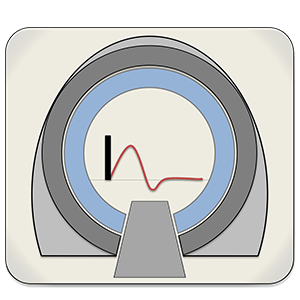
\includegraphics[width=.3\textwidth]{fig/de_icon.png}
	\end{center}
	\vspace*{\fill}
	\flushright{version 2016-10-27.1709}
\end{titlepage}
\newpage

%%%%%%%%%%%%%%%%%%%%%%%%%%%%%%%%%%%%%%%
%%%%%%%%%% Table of Contents %%%%%%%%%%
%%%%%%%%%%%%%%%%%%%%%%%%%%%%%%%%%%%%%%%

\hypersetup{
	linkcolor=black,
	}
\pagenumbering{Roman}
\tableofcontents
\label{sec:toc}
\newpage

%%%%%%%%%%%%%%%%%%%%%%%%%%%%%
%%%%%%%%%% Figures %%%%%%%%%%
%%%%%%%%%%%%%%%%%%%%%%%%%%%%%

\listoffigures
\newpage

%%%%%%%%%%%%%%%%%%%%%%%%%%%%%
%%%%%%%%%% Preface %%%%%%%%%%
%%%%%%%%%%%%%%%%%%%%%%%%%%%%%

% header and footer stuff
\renewcommand{\footrulewidth}{0.5pt}
\rhead{\vspace*{\fill} Page \thepage}
\cfoot{\vspace*{\fill}\href{https://en.wikipedia.org/wiki/Haemodynamic_response}{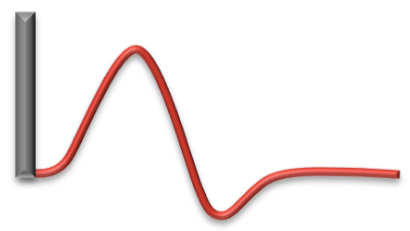
\includegraphics[scale=0.1]{fig/hrf.jpg}}}
% counters
\setcounter{page}{1}
\setcounter{section}{1000}
\section{Preface}
\label{sec:pref}
	Say you, an enthusiastic, young cognitive neuroscientist, have an archaic research question such as, ``Where in the brain responds more selectively to faces compared to other stimuli?''
	After all, humans are experts at quickly recognizing faces, so there must be specific cortical architecture and resources dedicated to face processing, right?
	Say you haven't done a proper literature search and found \shortciteNP{kanwisher1997fusiform} or you EVEN missed the compelling response by \shortciteNP{Haxby:Science:2001} that casts doubt onto the previous finding that there even IS such a brain module.
	All experiments in this workbook will be constructed to address this research question while slowly adding complexity to your experimental design.

	This document is designed to be an instructive tool that illustrates functional magnetic resonance imaging (fMRI) experimental design using the fMRI Design Explorer. 
	For Unit 1, It is assumed that you have the program in working order and that the program is open and ready to build an experiment.
	The \hyperref[sec:install]{installation} section will provide you all system requirements, dependencies, and installation steps.
	You can save your progress in an experiment file and return at a later time.
	This workbook is meant to accompany PSYC 411 / PSYC 888P / NACS 728F - \textit{Introduction to Functional Magnetic Resonance Imaging} at the University of Maryland - College Park, however, it can be useful to any who wish to begin using the fMRI Design Explorer program for all of their fMRI experimental design needs. 
	\bibliographystyle{apacite}
	\bibliography{workbook}
\newpage

%%%%%%%%%%%%%%%%%%%%%%%%%%%%%%%%%%
%%%%%%%%%% Introduction %%%%%%%%%%
%%%%%%%%%%%%%%%%%%%%%%%%%%%%%%%%%%

% change link colors
\hypersetup{
	linkcolor=PineGreen,
	urlcolor=RoyalBlue
	}
\section{Introduction}
\label{sec:into}
	\subsection*{About this workbook}
	\label{subsec:intro.manu}
		This workbook provides an interactive and comprehensive description of the functionality of the fMRI Design Explorer.
		When this PDF is viewed electronically, it offers a number of helpful internal and external hyperlinks.
		In addition, hovering over the hyperlink with a mouse should result in a preview of the link's content.
		These hyperlinks have been tested on both Mac OS X and Linux operating systems.
		However, individual operating system and PDF viewer idiosyncrasies may prevent functional hyperlinks.
		Please report all hyperlink issues to Dustin Moraczewski at \href{mailto:dmoracze@umd.edu}{dmoracze@umd.edu}.

		\subsubsection*{Internal Hyperlinks}
		\label{subsubsec:internal}
			Hyperlinks colored \textcolor{PineGreen}{green} refer to internal links.
			Clicking an internal link will navigate the PDF to the corresponding section or figure.
			For example, if the text refers to \hyperref[fig:launch]{Figure \ref{fig:launch}}, clicking on this link will navigate the PDF to Figure 1.
			In addition, the \hyperref[sec:toc]{Table of Contents} is fully interactive, however (as you probably noticed) the text color is not \textcolor{PineGreen}{green}.
			This decision was made for readability.

		\subsubsection*{External Hyperlinks}
		\label{subsubsec:external}
			Hyperlinks colored \textcolor{RoyalBlue}{blue} refer to external links.
			Clinking an external link will initiate behavior external to the PDF.
			There are three types of external links:
			\begin{enumerate}
				\item URL link - this will open a browser and navigate to a specific URL.
				\item Email link - this will open an email client, if one is configured (currently does not work on the University of Maryland's GLUE network)
				\item Download link - this will download relevant files (e.g. the Design Explorer installer).
				This link may also open a browser that navigates to Dropbox on certain operating systems.
			\end{enumerate}
			For example, if the text refers to the \href{https://afni.nimh.nih.gov}{AFNI} package for fMRI analysis, clicking on the corresponding link will open a browser that navigates to the AFNI homepage.
\newpage

%%%%%%%%%%%%%%%%%%%%%%%%%%%%%%%%%%%%%%%%%%%%%%%%%%%%%%%
%%%%%%%% Installation and System Requirments %%%%%%%%%%
%%%%%%%%%%%%%%%%%%%%%%%%%%%%%%%%%%%%%%%%%%%%%%%%%%%%%%%

\section{Download and Installation}
\label{sec:install}
	\subsection*{System Requirements}
	\label{subsec:reqs}
		64-bit machines running Mac OS X and Linux have been tested. \\
		It is likely that the program will run on others and may fail with some. \\ \\
		Windows operating system is not supported.

		\subsubsection*{Dependencies}
		\label{subsubsec:depend}
			Mac OS X -- \href{https://www.xquartz.org}{XQuartz} is required. \\
			Linux -- no dependencies.

	\subsection*{Download}
	\label{subsec:dl}
		Please download the current Design Explorer installer \href{https://www.dropbox.com/s/ncyeid1en3vjg57/DesignExplorer_installer?dl=1}{here}.

	\subsection*{Install}
	\label{subsec:install}
		\begin{enumerate}
			\item Open Terminal console.
			\item Navigate to the directory that contains the installer.
\begin{lstlisting}
> cd <path_to_installer>
\end{lstlisting}
			\item Change installer to executable, changing the version number appropriately.
\begin{lstlisting}
> chmod 755 Install_DesignExplorer_XXXX-XX-XX.XXXX
\end{lstlisting}
			\item Run the installer.
\begin{lstlisting}
> ./InstallDesignExplorer
\end{lstlisting}
			\item Pay attention to the output in the terminal.
			If there is an error, you should report this text to the developers.
			\item Once the installer is finished, an executable file called \texttt{DesignExplorer} will be deposited into your home (\texttt{\textasciitilde}) directory.
		\end{enumerate}

	\subsection*{Run}
	\label{subsec:run}
		\begin{enumerate}
		\item To run the Design Explorer you can either double click on the \texttt{DesignExplorer} file OR you can run the program in the terminal:
\begin{lstlisting}
> ~/DesignExplorer
\end{lstlisting}
		\end{enumerate}
		The executable file \texttt{DesignExplorer} is a bash script that points to a \texttt{\textasciitilde/.DesignExplorer} hidden directory that contains a python distribution, all dependencies, \href{https://afni.nimh.nih.gov/pub/dist/doc/program_help/3dDeconvolve.html}{AFNI's 3dDeconvolve}, and the \hyperref[subsec:default]{default project}.

	\subsection*{Uninstall}
	\label{ininstall}
		To uninstall the Design Explorer, simply open the terminal and type:
\begin{lstlisting}
> rm -rf ~/.DesignExplorer
\end{lstlisting}
		Be aware, though, that this will also delete the \hyperref[subsec:default]{default project} as well. \\
		\vfill
		Please email \href{mailto:dmoracze@umd.edu}{Dustin Moraczewski} with any issues related to installation.
		Be sure to be as descriptive as possible and provide your system configuration, what you did, and what was the output.
\newpage

%%%%%%%%%%%%%%%%%%%%%%%%%%%%%%
%%%%%%%%%% Overview %%%%%%%%%%
%%%%%%%%%%%%%%%%%%%%%%%%%%%%%%

\section{Overview of Program}
\label{sec:overview}
	To see the forest rather than jumping right to the trees, this section gives users a quick overview of the multiple large-scale features of the Design Explorer.
	In addition, this section provides tips on \hyperref[subsec:start]{getting started}, some \hyperref[subsec:general]{general information}, and an \hyperref[subsec:overview]{overview of the interface}.

	\subsection*{Getting Started}
	\label{subsec:start}
		Upon \hyperref[subsec:run]{executing} the Design Explorer, the Project Launcher window will appear:
		\vspace{3mm}
		\begin{figure}[ht]
		\centering
		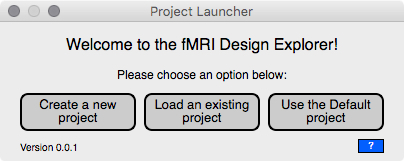
\includegraphics[width=0.4\textwidth,frame]{fig/1_launcher.jpg}
		\caption{Project Launcher}
		\label{fig:launch}
		\end{figure}

		Users have a three choices regarding how they want to initialize a project:
		\begin{enumerate}
			\item \hyperref[subsubsec:new]{Create a new project}
			\item \hyperref[subsubsec:load]{Load an existing project}
			\item \hyperref[subsec:default]{Use the Default  project}
		\end{enumerate}

		\subsubsection*{Create a new project button}
		\label{subsubsec:new}
			To create a new project within a user-defined location, choose this option. 
			A file directory dialog window will appear and the user will need to choose a location for their new project.
			Typically, prior to the creation of a new project, users will create a unique directory for their project.
			This unique directory will ensure that all files relevant to the project are contained within a single location.
			\begin{enumerate}
				\item Choose the \textbf{Create a new project} button
				\item Navigate to desired directory
				\item Click \textbf{choose}
				\item Enter project name
				\item Click \textbf{ok}
			\end{enumerate}

			The new project will be created and the main window will appear (\hyperref[fig:overview]{Figure \ref{fig:overview}}).

		\subsubsection*{Load an existing project button}
		\label{subsubsec:load}
			If a previous project had been created within a user-defined location (using the \hyperref[subsubsec:new]{Create a new project} button), users can choose to load this already existing project.
			\begin{enumerate}
				\item Choose the \textbf{Load an existing project button}
				\item Navigate to project's directory
				\item Click \textbf{choose}
			\end{enumerate}

			The project will load where the user left off, including all variants.

		\subsubsection*{Use the Default project button}
		\label{subsec:default}
			The default project exists so that users can rapidly create and interact with experimental designs without cluttering up the file system.
			Upon initialization of the default project, the Design Explorer will deposit a directory called \texttt{default\_project} within the \texttt{\textasciitilde/.DesignExplorer} directory and the user will be asked to name the project.
			If a default project already exists, clicking the \textbf{Use the Default project} button will open the previously saved default project.

			To remove the default project, open a terminal and type:
\begin{lstlisting}
> rm -rf ~/.DesignExplorer/default_project
\end{lstlisting}

	\subsection*{General Information}
	\label{subsec:general}

		\subsubsection*{Autosave}
		\label{subsubsec:save}
			All changes within a valid design are autosaved, thus, there is no need to save manually.
			However, there is a caveat to the autosave feature: in order for changes to be saved, the changes must occur within a valid design and be valid with respect to the parameters of interest.
			For example, the autosave feature will not save changes under the following scenarios:
			\begin{enumerate}
				\item If events are defined and/or configured without first creating a design using the \nbut{} button, the changes will be lost because they did not occur within the context of a design.
				\item Entering a character instead of a number into the \textbf{TR} field would not be saved since this field expects a numeric value.
			\end{enumerate}

			These scenarios are meant to represent the types of behaviors that would fail to autosave and do \textbf{not} encompass all possibilities.

	\subsection*{Overview of Interface}
	\label{subsec:overview}
		This section gives a brief overview of the main interface that is common to all Tabs.
		Please see the \hyperref[subsec:tabs]{Tabs} section for functionality unique to each Tab.
		\hyperref[fig:overview]{Figure \ref{fig:overview}} depicts the large-scale structure of the Design Explorer interface.
		\begin{figure}[ht]
			\centering
			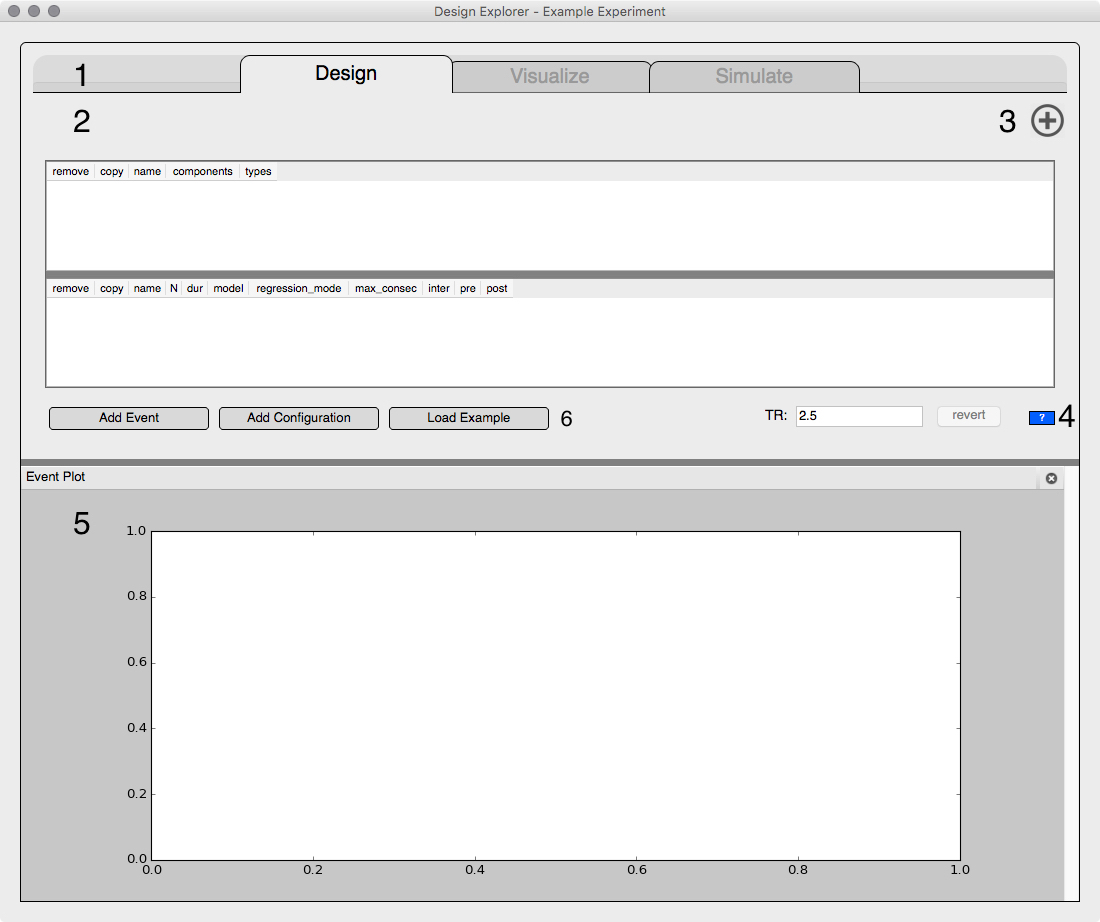
\includegraphics[width=0.75\textwidth,frame]{fig/2_overview.jpg}
			\caption{Overview of Interface}
			\label{fig:overview}
		\end{figure}

		Consider the number annotations in \hyperref[fig:overview]{Figure \ref{fig:overview}}:
		\begin{enumerate}
			\item The \hyperref[subsec:tabs]{Tab} menu: \\
			This menu consists of the main functional divisions of the Design Explorer.
			The tabs consist of \hyperref[subsubsec:design]{Design}, \hyperref[subsubsec:visualize]{Visualize}, and \hyperref[subsubsec:simulate]{Simulate}.
			\item The Design menu: \\
			This menu consists of the user-defined designs currently in the workspace.
			In \hyperref[fig:overview]{Figure \ref{fig:overview}}, this menu is currently blank which means that no designs have been created yet.
			A design must be created before defining or configuring events.
			\item The New Design button \nbut{}: \\
			This button adds a new design to the Design Menu.
			When this button is clicked, users will be asked to enter a name for the new design.
			All designs must have unique names.
			\item The \hyperref[subsubsec:hbut]{Help Button} \hbut{} \\
			This button is available in all three tabs.
			\item The Plot window: \\
			This window is available in all tabs, however, the information presented within this window is unique to each tab.
			For example, the plot window in the \hyperref[subsubsec:design]{design tab} shows the event plots whereas this window in the \hyperref[subsubsec:visualize]{visualize} and \hyperref[subsubsec:simulate]{simulate} tabs show the ideal and simulated BOLD signal, respectively.
			\item The \hyperref[subsubsec:example]{Load Example button}: \\
			Click this button to load specific examples from this workbook.  
		\end{enumerate}

	\subsection*{Tabs}
	\label{subsec:tabs}
		This section gives a brief, big-picture overview of the functionality of each of the tabs. Please see the corresponding chapters for greater detail regarding the implementation of the features.

		\subsubsection*{Design}
		\label{subsubsec:design}
			The purpose of the Design tab is three-fold:
			\begin{enumerate}
				\item Define events into an event hierarchy
				\item Configure the various parameters of the events
				\item View experimental design as an event plot
			\end{enumerate}

			There are multiple ways in which users can define their event hierarchy, see the Event Hierarchy chapter for more information.
			With regards to event configuration, users have complete control of most parameters: number of events, event duration, hemodynamic response models, maximum consecutive events of the same type, pre, inter, and post baseline periods.
			Both events convolved with a hemodynamic response and not are configurable.

		\subsubsection*{Visualize}
		\label{subsubsec:visualize}
			The purpose of the visualize tab is to view the idealized (no noise added) BOLD signal on your experiment.
			Users can also view event-specific signal to examine the relative contributions of each event to the overall BOLD signal.
			This signal is derived from the events that are configured to include a hemodynamic response model.
			In addition, the Event Configuration table is also supplied so that users can make adjustments to the event parameters and see the changes in the BOLD signal in real time.

		\subsubsection*{Simulate}
		\label{subsubsec:simulate}
			The purpose of the Simulate tab is to use an experimental design to simulate BOLD signal according to user-defined event-specific $\beta$ weights, event-specific noise, as well as global noise.
			Then, once new BOLD signal is simulated, users can examine the error in the recovered $\beta$ estimates.
			The number of simulations is a user-defined parameter.

	\subsection*{Help}
	\label{subsec:help}
		\subsubsection*{The Load Example Button}
		\label{subsubsec:example}
			The load example button is a quick and easy way to load the designs discussed in the units of the workbook.
			Thus, users can load an example quickly and begin interacting with the designs without spending time defining and configuring each individual event.
		\subsubsection*{The Help Button}
		\label{subsubsec:hbut}
			The help button \hbut{}, as seen in the lower right corner of \hyperref[fig:launch]{Figure \ref{fig:launch}}, will open this user manual to provide further assistance on the implications of these decisions.
			This button is available in the \hyperref[fig:launch]{Project Launcher}, \hyperref[subsubsec:design]{Design tab}, \hyperref[subsubsec:visualize]{Visualize tab}, and \hyperref[subsubsec:simulate]{Simulate tab}.

		\subsubsection*{Debug Windows}
		\label{subsubsec:debug}
			In the current version, initializing the Design Explorer will also open two other windows: a terminal window and a debug window.
			Each of these windows provides different information about the background processes.
			Overall, these windows are not necessary to keep in view, however, if there are any errors or the program is not behaving as you expected it, the out put of these windows can help.

		\subsubsection*{Further Assistance}
		\label{subsubsec:furtherhelp}
			If you find a bug, please \href{mailto:dmoracze@umd.edu}{Dustin Moraczewski} with a description of what happened and any text you see in these windows.
			In the interest of fixing all bugs, the more information provided to the developers the better.
			A detailed description of what you did, screen shots, and debug and terminal window text would provide a helpful overview in order to diagnose what happened.
\newpage

%%%%%%%%%%%%%%%%%%%%%%%%%%%%
%%%%%%%%%% Unit 1 %%%%%%%%%%
%%%%%%%%%%%%%%%%%%%%%%%%%%%%
\pagenumbering{arabic}
\renewcommand{\thesubsection}{\arabic{section}.\arabic{subsection}}
\section{Unit 1: The Hemodynamic Response}
\label{sec:unit1}
\setcounter{section}{1}
	\subsection{Overview}
	\label{subsec:u1overview}
		Before constructing an experiment, we must first understand how specific, transient events could be reflected in neurobiological terms.
		The hemodynamic response in the brain is slow relative to action potentials at the single-neuron and neural-population level.
		Therefore, this unit will give you the intuition of how events, which are computed by the brain at the neural level, translate to increased metabolic activity to replenish oxygen to the neural cell bodies.

	\subsection{Define and Configure Events}
	\label{subsec:u1define}
		First we will explore how a single, transient event elicits a hemodynamic response.
		Here we are making an assumption that there is a one-to-one correspondence between the hemodynamic response and the event in question, say the presentation of a picture of a face.
		This is an ideal example for educational purposes, and in practice real data are far more variable.
		We will begin by setting up the stimulus presentation so that we can build a larger experiment from this template in later units. \\ \\
		When defining events, it is helpful to think about hierarchies.
		In the current example, our event hierarchy will look like \hyperref[fig:single_stim_heirarchy]{Figure \ref{fig:single_stim_heirarchy}}. 
		More on event hierarchies in Unit 2.
		\begin{figure}[ht]
			\centering
			\begin{tikzpicture}[every tree node/.style={align=center,minimum width=\widthof{run}}]
				\Tree 
 				[ .{run}
   					[ .{trial} 
     						[ .{stimulus} ] ] 
   					[ .{post} ] ]
			\end{tikzpicture}
			\caption{Single stimulus event hierarchy}
			\label{fig:single_stim_heirarchy}
		\end{figure} \\
		Now let's build it.
		For the purposes of this workbook, column names (see below) will be in \textbf{bold} and text that needs to be entered into text boxes will be in ``quotes''.
		Begin in the \hyperref[subsubsec:design]{Design} tab to construct your experiment:
		\begin{figure}[ht]
			\centering
			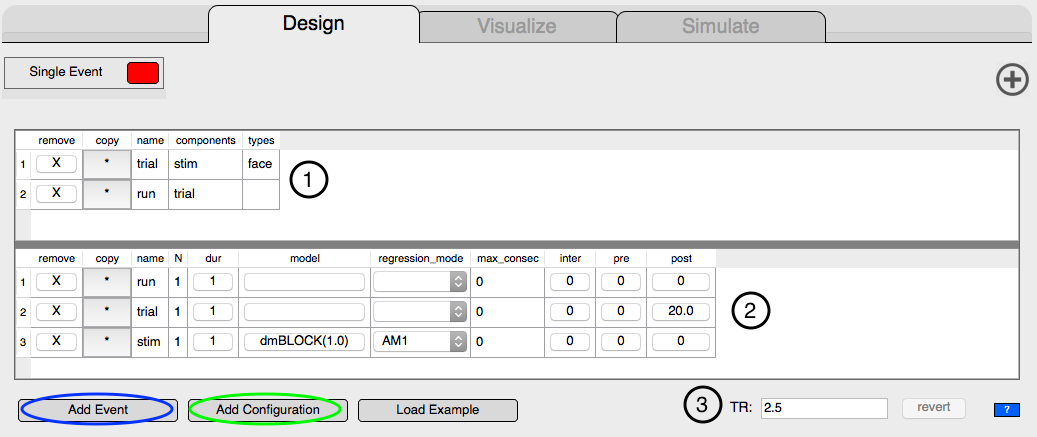
\includegraphics[width=0.95\textwidth,frame]{fig/04_single_event_design.jpg}
			\caption{Single stimulus event configuration}
			\label{fig:single_stim_config}
		\end{figure}
		\begin{enumerate}
			\item Click the \textbf{New Design} button \nbut{}
			\item Enter ``Single Event'' as the name of the design, click \textbf{ok}
			\item Add events to your experiment by clicking \textbf{Add Event} (\hyperref[fig:single_stim_config]{Figure \ref{fig:single_stim_config}}, \textcolor{blue}{\textbf{blue}} circle), which will insert a column in the Event Definition table (\hyperref[fig:single_stim_config]{Figure \ref{fig:single_stim_config}}, \circled{1}). You will add two different parts to your experiment: ``run'' and ``trial''.
			Add ``run'' and ``trial'' in to the \textbf{name} column of the first and second rows of the table, respectively.
			While these two events are not immediately applicable to a presentation of one stimulus, it will become clear once we expand the complexity of the experiment.
			\item Next continue to define the events in the Event Definition table.
			The run event will consist of a \textbf{component} named ``trial''. Intuitively, this illustrates that within the run event you will have smaller events called trials.
			For the trial Event (row 2 of the Event Definition Table) the \textbf{component} will be named ``stimulus'' and we will define one \textbf{type}: ``face''.
			This definition is saying that within each run we will have events called trials.
			With each trial we will have events called ``stimulus'', and, for this setup, we will only have one type of stimulus: ``face''.
			``stimulus'' will correspond to the onset of each face presentation.
			\item Now we need to configure our events.
			Keep in mind that we are constructing a special case of an experiment that only has one stimulus presentation, we will build on this design in later units.
			Click the \textbf{Add Configuration} button (\hyperref[fig:single_stim_config]{Figure \ref{fig:single_stim_config}}, \textcolor{green}{\textbf{green}} circle) to insert a line into the Configure Events table (\hyperref[fig:single_stim_config]{Figure \ref{fig:single_stim_config}}, \circled{2}).
			We will need to insert 3 rows into this table, corresponding to ``run'', ``trial'', and ``stimulus''.
			Enter each of these into the \textbf{name} column, respectively.
			It does not matter which order these rows are in, however, it is essential that the text in the \textbf{name} column be identical to the events in the Event Definition table.
			\begin{enumerate}
				\item For the run configuration, we can use all of the defaults, except for \textbf{post} which denotes a post-run event where the participant views a fixation cross for a defined period of time.
				For this example, enter a post-run fixation event of 20 seconds.
				\item For the trial configuration, we can use the default settings.
				\item For the stimulus configuration, we will use the defaults except that we need to define a hemodynamic response model with which to convolve the event. In the \textbf{model} column, we will select \textbf{dmBLOCK} with an amplitude of 1. We also need to select a \textbf{regression\textunderscore mode} of AM1. 
				AM stands for amplitude modulation, which means that the height of the hemodynamic response will be dictated by the value entered int the dmBLOCK model specification.
				More on different types of models will be discussed later.
			\end{enumerate}
			\item For example purposes, we will also change the \textbf{TR} (repetition time) to an unrealistic 0.01 seconds (\hyperref[fig:single_stim_config]{Figure \ref{fig:single_stim_config}}, \circled{3}).
			You will explore the effects of a changing TR on the response behavior in the unit exercises.
		\end{enumerate}
		\begin{figure}[ht]
			\centering
			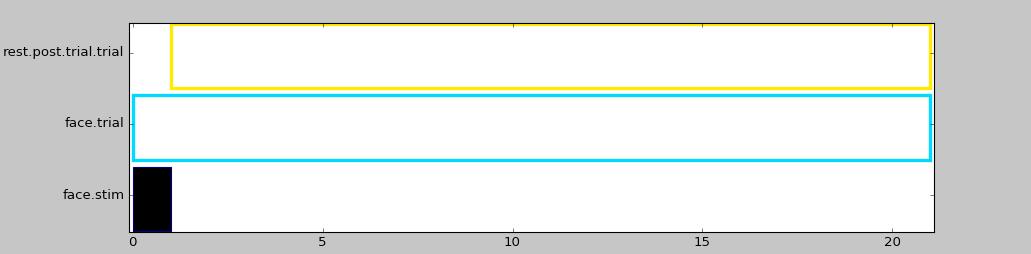
\includegraphics[width=0.70\textwidth,frame]{fig/05_single_event_design_plot.jpg}
			\caption{Single stimulus event plot}
			\label{fig:single_event_plot}
		\end{figure}
		Once you have defined and configured your events, your single-stimulus experiment should look like \hyperref[fig:single_event_plot]{Figure \ref{fig:single_event_plot}}.
		In this plot, we can see a graphical illustration of the events in our experiment with events on the Y-axis and time in seconds on the X-axis.
		The top line (empty \textcolor{Goldenrod}{\textbf{yellow}} box) represents the 20 second post-run fixation we entered under the Run event.
		The second line (empty \textcolor{cyan}{\textbf{cyan}} box) denotes the trial event we defined.
		Finally, the solid \textbf{black} box shows the actual presentation of the stimulus.
		Events are depicted as either empty or solid boxes.
		Empty boxes correspond to events where we are not going to estimate the hemodynamic response whereas solid events are events where we will estimate this effect (the manner in which we estimate the response is set using the \textbf{model} and \textbf{regression\textunderscore mode} columns of the Event Configuration table).

	\subsection{Visualize Event Signal}
	\label{subsec:u1viz}
		Now that we defined and configured the events in our simple design, we can now visualize the translation of these events into a hemodynamic response.
		Keep in mind that this is an idealized example.
		\textit{In a perfect world}, these response plots depict that a presentation of a face elicits an \textit{ideal} hemodynamic response - real experimental data are never this clean. \\ \\
		To view the response plots, click the \hyperref[subsubsec:visualize]{Visualize} tab (\hyperref[fig:single_stim_viz_config]{Figure \ref{fig:single_stim_viz_config}}, \textcolor{blue}{\textbf{blue}} circle):
		\begin{figure}[ht]
			\centering
			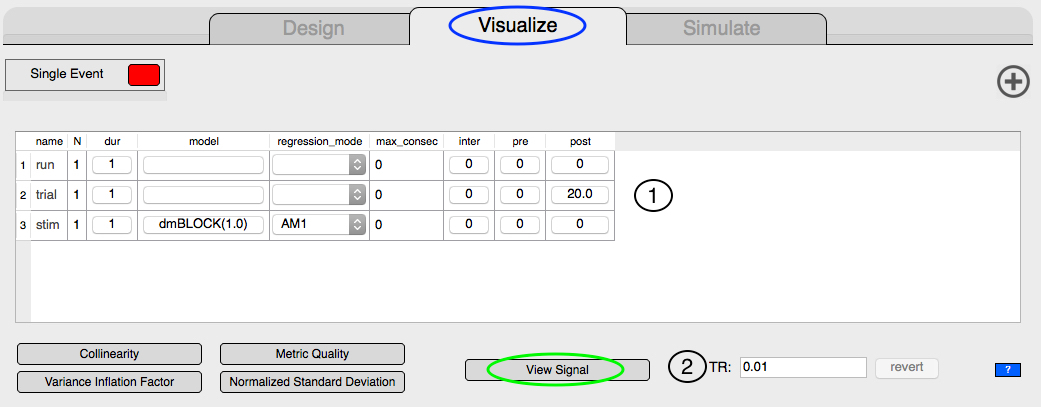
\includegraphics[width=0.95\textwidth,frame]{fig/06_single_event_visualize_config.jpg}
			\caption{Single stimulus visualize configuration}
			\label{fig:single_stim_viz_config}
		\end{figure} \\
		Just as in the \hyperref[subsubsec:design]{Design} tab (\hyperref[fig:single_stim_heirarchy]{Figure \ref{fig:single_stim_heirarchy}}), \hyperref[fig:single_stim_viz_config]{Figure \ref{fig:single_stim_viz_config}}, \circled{1}, shows the Event Configuration table that you created earlier.
		Here you will be able to edit the event parameters and visualize how the hemodynamic response changes based on your design changes.
		You can also change the TR length in \hyperref[fig:single_stim_viz_config]{Figure \ref{fig:single_stim_viz_config}}, \circled{2}.
		To visualize the ideal hemodynamic response of the defined events, click \textbf{signal} button (\hyperref[fig:single_stim_viz_config]{Figure \ref{fig:single_stim_viz_config}}, \textcolor{green}{\textbf{green}} circle).
		\begin{figure}[ht]
			\centering
			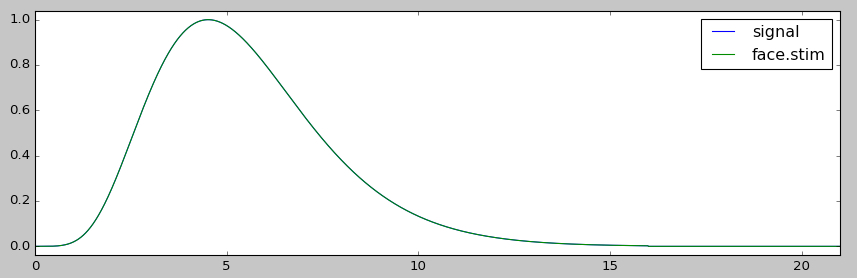
\includegraphics[width=0.70\textwidth,frame]{fig/07_single_event_visualize_plot.jpg}
			\caption{Single stimulus hemodynamic response}
			\label{fig:single_stim_HRF}
		\end{figure} \\
		\hyperref[fig:single_stim_HRF]{Figure \ref{fig:single_stim_HRF}} shows the hemodynamic response corresponding to the events in the experiment.
		Time is on the X-axis and hemodynamic amplitude (the strength of the response) is on the Y-axis.
		Time 0 would correspond to the onset of the 1-second long stimulus. 
		Note that the peak of the hemodynamic response is at roughly the 5 second mark, which should be consistent with what you have learned about the time course of the response.
		Now that you have configured the events and can visualize the corresponding response, you are now equipped to explore the end of the unit exercises.
		\newpage

	\subsection{Unit Exercises}
	\label{subsec:u1exercises}
		\begin{enumerate}
			\item Change the TR to a more realistic 2.5 seconds. How does the response change and why?
			\item Change the TR to .1, 1, 2, 3, 5, 8, and 13. What happens as the TR length increases? Pay attention to the shape of the curve.
			\item What happens to the amplitude as you go from 5, 8, and 13 second TRs? Why?
			\item Change the TR back to 0.01 seconds. Now change the duration of the stimulus to 3, 5, 8, and 13 seconds. How does the response change and why?
			\item Reset the stimulus duration to 1 second and remove the post Run fixation period (set to 0). How does the response change and why?
			\item Reset the post Run fixation period to 20 seconds. Now change the number of Stimulus presentations from 1 to 2. How does the response and amplitude change? Is this what you expected? why?
			\item Now change the \textbf{inter-stimulus interval} (ISI, the amount of time between stimulus presentations) to 3, 5, 8, and 13. How does the shape and amplitude of the response change?
			\item Say you want a proper control for your study.
			You realize that comparing the presentation of a face to baseline (a fixation cross) does not isolate brain regions that solely respond to faces.
			In a faces vs. baseline comparison there are also low-level visual differences in luminance, contrast, edges, and complexity of the visual stimuli.
			To further control for these effects you decide to show a scrambled image as well.
			These scrambled images will have the same luminance, contrast, edges, and complexity as the face stimuli, but they will not be in the form of a face.
			Thus, you want to add a new condition: Scrambled.
			\begin{enumerate}
				\item Return to the \hyperref[subsubsec:design]{Design} tab (\hyperref[fig:single_stim_config]{Figure \ref{fig:single_stim_config}}).
				\item Add another \textbf{Type} (separated from ``face'' with a comma i.e. ``face,scrambled'') to the trial event called: ``scrambled'', \hyperref[fig:single_stim_config]{Figure \ref{fig:single_stim_config}}, \circled{1}.
				\item In the Event Configuration table (\hyperref[fig:single_stim_config]{Figure \ref{fig:single_stim_config}}, \circled{2}), set the number of stimulus events to 2.
				\item Return to the \textbf{Visualize} tab (\hyperref[fig:single_stim_viz_config]{Figure \ref{fig:single_stim_viz_config}}, \textcolor{blue}{\textbf{blue}} circle) and view the new signal (\hyperref[fig:single_stim_viz_config]{Figure \ref{fig:single_stim_viz_config}}, \textcolor{green}{\textbf{green}} circle).
			\end{enumerate} 
			What does the overall signal (\textcolor{blue}{blue} line) look like? Can we differentiate the two conditions from this signal? Change the \textbf{Inter-Trial Interval} (ITI, space between trials) to 1, 3, 5, 8, and 13 seconds. How does this change affect the overall shape and amplitude of the signal?
	 	\end{enumerate}
\newpage

%%%%%%%%%%%%%%%%%%%%%%%%%%%%
%%%%%%%%%% Unit 2 %%%%%%%%%%
%%%%%%%%%%%%%%%%%%%%%%%%%%%%
\section{Unit 2: Event Hierarchy}
\label{sec:unit2}
	\subsection{Overview}
	\label{subsec:u2overview}
		When building an experiment, it can be useful to think of each event as nested within an event hierarchy rather than a series of independent events.
		It is not only conceptually useful, it is how experiments are defined in the fMRI Design Explorer.
		The program then uses this hierarchy to optimize stimulus timing, which makes the world a better place.
		This unit will explain how to think of an experiment as a hierarchy of events and how to define that hierarchy in the Design Explorer.

	\subsection{Hierarchy Outlined}
	\label{subsec:u2outline}
		In our face viewing experiment we can think of two types of events: when a stimulus is on the screen and when the screen is blank (the inter-trial interval).
		Now, imagine that every single face presentation is independent of each ITI, that is, no stimulus is bound to an ITI.
		The event structure of this experiment would look something like \hyperref[fig:no_hierarchy]{Figure \ref{fig:no_hierarchy}}.
		\begin{figure}[ht]
			\centering
			\begin{tikzpicture}[every tree node/.style={align=center,minimum width=\widthof{run}}]
				\Tree 
	 			[ .{experiment}
	   				[ .{stimulus} ]
	     				[ .{iti} ]
	     				[ .{stimulus} ]
	     				[ .{iti} ] 
	     				[ .{stimulus} ]
	     				[ .{iti} ]
	     				[ .{stimulus} ]
	     				[ .{iti} ]]
			\end{tikzpicture}
			\caption{Minimal Hierarchy}
			\label{fig:no_hierarchy}
		\end{figure}
		However, there is a practical constraint to a ``minimal hierarchy'' design - typical fMRI experiments last more than one functional run.
		Researchers like to exert control over their experiments and so, to ensure that there is no unintended effect of run on the data, runs are typically counterbalanced across participants.
		This means that the order in which the runs are presented to participants is shuffled.
		In a two run experiment (with runs A and B), some participants will receive run A first whereas some participants will receive run B first.
		It is important to ensure that each run is not significantly different from other runs with regard to the number of trials and timing.
		Thus, we can think about the stimulus and ITI events as occurring \textit{within} each run.
		The event structure of an experiment that considers stimuli and ITI as nested within run is depicted in \hyperref[fig:run_hierarchy]{Figure \ref{fig:run_hierarchy}}.
		\begin{figure}[ht]
			\centering
			\begin{tikzpicture}[every tree node/.style={align=center,minimum width=\widthof{run}}]
				\Tree 
	 			[ .{experiment}
	 				[ .{run}
	   					[ .{stimulus} ]
	     					[ .{iti} ]
	     					[ .{stimulus} ]
	     					[ .{iti} ] ]
					[ .{run}
	     					[ .{stimulus} ]
	     					[ .{iti} ]
	     					[ .{stimulus} ]
	     					[ .{iti} ] ] ]
			\end{tikzpicture}
			\caption{Run Level}
			\label{fig:run_hierarchy}
		\end{figure}
		While this ensures that each run is independent, there are still many problems with constructing your experiment in this manner.
		If we randomized the order of the run event in \hyperref[fig:run_hierarchy]{Figure \ref{fig:run_hierarchy}}, we could still counterbalance runs and test to ensure that runs did not differ in timing.
		However, we also want to make sure that the order of stimulus presentation does not affect our results.
		While the above examples only have 4 stimulus events (2 per run), keep in mind that the typical experiment has many more.
		We want to ensure that there are no systematic effects with respect to stimulus timing.
		For example, we want to make sure that participants cannot predict what trial will be next or else expectancy effects could influence the results in unintended ways.
		If we were to randomize the stimulus and ITI events in \hyperref[fig:run_hierarchy]{Figure \ref{fig:run_hierarchy}} we would have a problem.
		We have the stimulus and ITI at the same level which means that we could potentially get two (or even three!) ITI events back to back, and the same goes for the stimulus events.
		We want to make sure that each stimulus is followed by an ITI, but we want to be able to randomize the stimulus.
		Thus, we can create a hierarchy like \hyperref[fig:trial_hierarchy]{Figure \ref{fig:trial_hierarchy}}:
		\begin{figure}[ht]
			\centering
			\begin{tikzpicture}[every tree node/.style={align=center,minimum width=\widthof{run}}]
				\Tree 
	 			[ .{experiment}
	 				[ .{run}
	   					[ .{trial}
	   						[ .{stimulus} ]
	     						[ .{iti} ] ]
						[ .{trial}
	     						[ .{stimulus} ]
	     						[ .{iti} ] ] ]
					[ .{run}
	   					[ .{trial}
	   						[ .{stimulus} ]
	     						[ .{iti} ] ]
						[ .{trial}
	     						[ .{stimulus} ]
	     						[ .{iti} ] ] ] ]
			\end{tikzpicture}
			\caption{Trial Level}
			\label{fig:trial_hierarchy}
		\end{figure}
		Here we are able to randomize run and trial order while ensuring that every stimulus is followed by an ITI event.

		\vspace{3mm}
		\textbf{NOTE: In the Design Explorer, the Experiment level of the above hierarchies is automatically defined and does not need to be included}

	\subsection{Hierarchy in the Design Explorer}
	\label{subsec:u2hierDE}
		Since the Design Explorer assumes a minimal run hierarchy, this is the level at which we can begin implementing hierarchical designs in the program.
		In the program, we will begin by building the experiment outlined in \hyperref[fig:run_hierarchy]{Figure \ref{fig:run_hierarchy}}. \\ \\
		To do this:
		\begin{enumerate}
			\item Begin in the \hyperref[subsubsec:design]{Design} tab
			\item Choose \textbf{New Design} button \nbut{}
			\item Enter ``Hierarchy'' as the name of this variant
			\item Click \textbf{ok}
		\end{enumerate}
		\begin{figure}[ht]
			\centering
			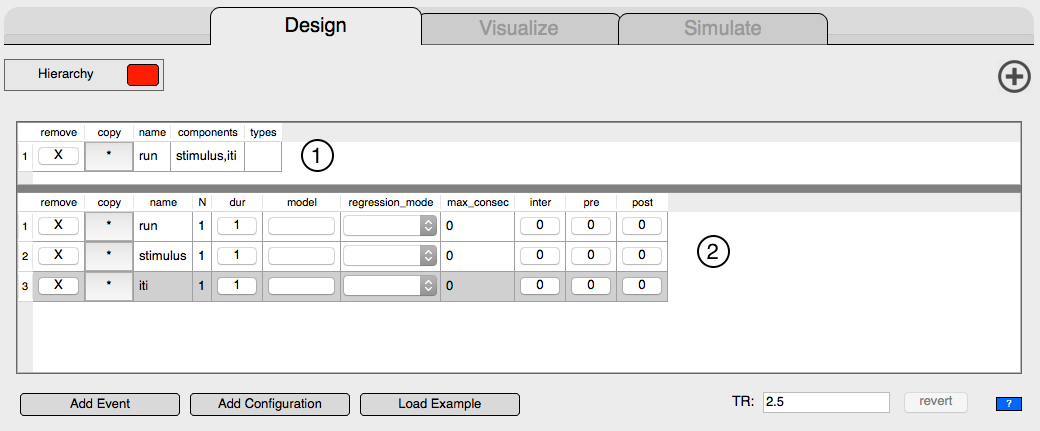
\includegraphics[width=0.95\textwidth,frame]{fig/08_run_level_config.jpg}
			\caption{Run Level Configuration}
			\label{fig:run_hierarchy_config}
		\end{figure}
		\begin{figure}[ht]
			\centering
			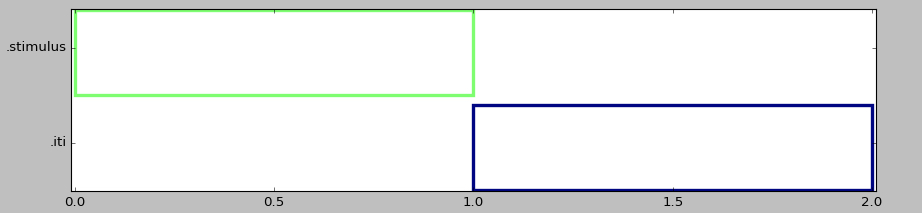
\includegraphics[width=0.70\textwidth,frame]{fig/09_run_level_event.jpg}
			\caption{Run Level Events}
			\label{fig:run_hierarchy_events}
		\end{figure}
		To build the design:
		\begin{enumerate}
			\item Click the \textbf{Add Event} button to add a row into the Event Definition Table (\hyperref[fig:run_hierarchy]{Figure \ref{fig:run_hierarchy}}, \circled{1})
			\item While the order of the rows does not matter, there must always be an event named run. Enter ``run'' into the \textbf{name} column of the first row in the Event Definition table
			\item In the \textbf{components} column of the run event, enter ``stimulus,iti''
			\item Click the \textbf{Add Configuration} button three times to add three rows into the Event Configuration table (\hyperref[fig:run_hierarchy]{Figure \ref{fig:run_hierarchy}}, \circled{2})
			\item Add ``run'', ``stimulus'', and ``iti'' into the \textbf{name} column for each of these events
		\end{enumerate}
		After you have defined and configured all events, your event plot should look like \hyperref[fig:run_hierarchy]{Figure \ref{fig:run_hierarchy_events}}.
		While this does not look like a very interesting experiment, it outlines the events you defined.
		The empty \textcolor{green}{\textbf{green}} box shows the event that corresponds to the stimulus, whereas the empty \textcolor{blue}{\textbf{blue}} box corresponds to the ITI event. \\
		Now that you have built this experiment, you can explore why this event organization is sub-optimal:

		\subsubsection*{Run Level Exercises}
		\label{subsubsection:run_hier_ex}
			\begin{enumerate}
				\item Change the number of stimulus and ITI events to 2, and then 3. 
				How did the event plot change?
				Is this what you would want to happen?
				\item To see the hierarchy in practice, change the number of runs to 2, and then 3.
				how did the event plot change?
			\end{enumerate}

		The experiment, as we have defined it, groups all like-events together.
		This is probably not what we would want out of an experiment because it makes no sense to have a group of stimuli followed by a group of ITI events. \\ \\
		In order to define a much more flexible experiment that knows to put an ITI event \textit{always} after a stimulus event, we need to implement the heirarchy as defined in \hyperref[fig:trial_hierarchy_config]{Figure \ref{fig:trial_hierarchy_config}}.
		\begin{figure}[ht]
			\centering
			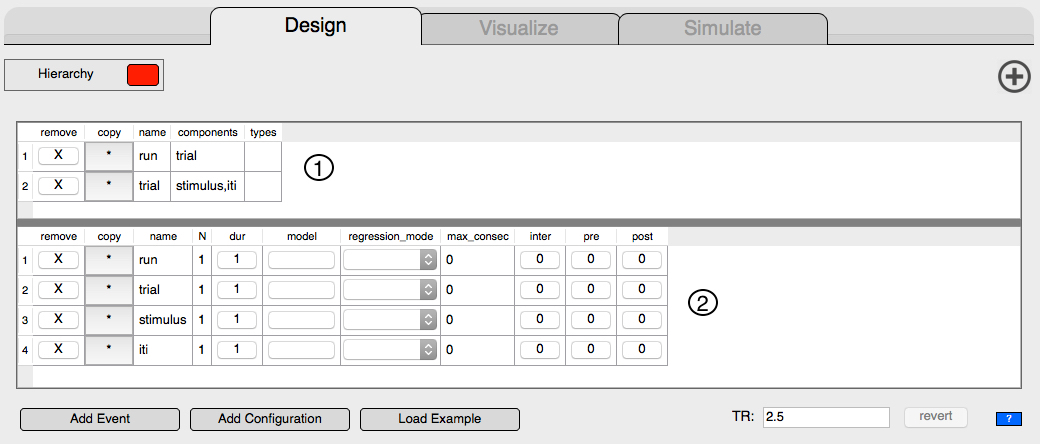
\includegraphics[width=0.95\textwidth,frame]{fig/10_trial_level_config.jpg}
			\caption{Trial Level Configuration}
			\label{fig:trial_hierarchy_config}
		\end{figure}
		\begin{figure}[ht]
			\centering
			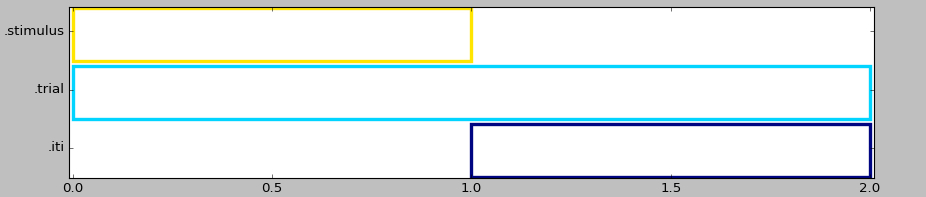
\includegraphics[width=0.70\textwidth,frame]{fig/11_trial_level_event.jpg}
			\caption{Trial Level Events}
			\label{fig:trial_hierarchy_events}
		\end{figure} \\
		In the \textbf{Design} tab:
		\begin{enumerate}
			\item Click the \textbf{Add Event} button to add a row into the Event Definition Table (\hyperref[fig:trial_hierarchy_config]{Figure \ref{fig:trial_hierarchy_config}}, \circled{1}).
			\item Enter ``run'' into the \textbf{name} column of the first row in the Event Definition table.
			\item In the \textbf{components} column of run, enter ``trial''.
			\item Add another row into this table. Under \textbf{name}, enter ``trial''.
			\item In the \textbf{componenets} of the trial event enter ``stimulus,iti''.
			Thus, for each ``run'' we will have events called ``trial'' and each ``trial'' event will consist of ``stimulus'' and ``iti''.
			\item Click the \textbf{Add Configuration} button four times to add four rows into the Event Configuration table (\hyperref[fig:trial_hierarchy_config]{Figure \ref{fig:trial_hierarchy_config}}, \circled{2}).
			\item You will need to name the rows the same as in the Event Definition table.
			Enter ``run'', ``trial'', ``stimulus'', and ``iti'' in the \textbf{name} column of the rows, respectively.
		\end{enumerate}

		Now that you have defined and configured the events in this hierarchy, your event plot should look like Figure~\ref{fig:trial_hierarchy_events}.
		You still have empty boxes for the stimulus (\textcolor{Goldenrod}{\textbf{yellow}} box) and ITI (\textcolor{blue}{\textbf{blue}} box) events.
		In addition, there is another empty box (\textcolor{Cyan}{\textbf{cyan}} box) that encompasses the stimulus and ITI events.
		This is the box that corresponds to the trial event.

		\subsubsection*{Trial Level Exercises}
		\label{subsubsection:trial_hier_ex}
			\begin{enumerate}
				\item Change the number of stimulus and ITI events to 2, and then 3. 
				How did the event plot change? Is this different than in the previous example?
				\item Change the number of stimulus and ITI back to 1.
				Now change the number of trials to 2, and then 3.
				How did the event plot change?
				\item Now add a post-run fixation period of 10 seconds to allow the hemodynamic response to return to baseline.
				To do this, there is no need to define another event, but rather you change the \textbf{post} column of the run row in the Event Configuration table.
				This will add a set amount of time after every run event.
			\end{enumerate}
	\newpage

	\subsection{Unit Exercises}
	\label{subsec:u2exercises}
		While some experiments can be as simple as a trial that consists of a stimulus and an ITI, many are more complicated.
		Take, for example, a classic monetary incentive delay task (\hyperref[fig:mid_hierarchy]{Figure \ref{fig:mid_hierarchy}}).
		In this experiment, participants can win money if their reaction time is fast enough on a button pushing task.
		Within each trial there is a cue where the participants are told what condition they are in (e.g. how much money they could win).
		This is followed by a delay period where they are waiting for the target.
		Then the target appears and participants must push a button as fast as they can (while holding still!).
		After the target, they are notified whether they pushed the button fast enough.
		Finally, this is followed by an ITI where participants are waiting for the next trial.
		Keep in mind that there are usually different trial types as well, this is where the \textbf{types} column of the Event Definition table will come in to play.
		\begin{figure}[ht]
			\centering
			\begin{scaletikzpicturetowidth}{\textwidth}
			\begin{tikzpicture}[scale=\tikzscale]
				\Tree 
	 			[ .{experiment}
	 				[ .{run}
	   					[ .{trial}
	   						[ .{cue} ]
	     						[ .{delay} ]
	     						[ .{target} ] 
	     						[ .{outcome} ]
	     						[ .{iti} ] ]
						[ .{trial}
	   						[ .{cue} ]
	     						[ .{delay} ]
	     						[ .{target} ] 
	     						[ .{outcome} ]
	     						[ .{iti} ] ] 
						[ .{post} ] ]
					[ .{run}
	   					[ .{trial}
	   						[ .{cue} ]
	     						[ .{delay} ]
	     						[ .{target} ] 
	     						[ .{outcome} ]
	     						[ .{iti} ] ]
						[ .{trial}
	   						[ .{cue} ]
	     						[ .{delay} ]
	     						[ .{target} ] 
	     						[ .{outcome} ]
	     						[ .{iti} ] ] 
						[ .{post} ] ] ]
			\end{tikzpicture}
			\end{scaletikzpicturetowidth}
			\caption{Monetary Incentive Delay Task Hierarchy}
			\label{fig:mid_hierarchy}
		\end{figure}
		\vspace{5mm}
		\begin{enumerate}
			\item Create an experiment in the Design Explorer that reflects the hierarchy in \hyperref[fig:mid_hierarchy]{Figure \ref{fig:mid_hierarchy}}.
			For this exercise, create 2 runs that consist of 2 trials each.
			Each trial will need a cue, delay, target, outcome, and ITI event.
			Finally, enter a post run fixation of 10 seconds after each run.
			While this exercise only includes 2 trials per run, keep in mind that there are many many more trials in a real experiment.
		\end{enumerate}
\newpage

%%%%%%%%%%%%%%%%%%%%%%%%%%%%
%%%%%%%%%% Unit 3 %%%%%%%%%%
%%%%%%%%%%%%%%%%%%%%%%%%%%%%

\section{Unit 3: Block Designs}
\label{sec:unit3}
	\subsection{Overview}
	\label{subsec:u3overview}
		In unit 1, we discussed how single, transient events can be translated into a hemodynamic response and how event duration, ITI, and other aspects can change the subsequent response.
		Then, in unit 2, we discussed how experiments can be thought of as hierarchical events and how to define these events in the Design Explorer.
		Now it is time to put these together and design your first experiment.
		Consider two properties of the hemodynamic response: 1) the hemodynamic response is slow compared to electrical activity at the neural level and 2) two (or more) events in quick succession will elicit a greater response (in terms of amplitude) compared to a single event.
		It would be beneficial to design an experiment that exploits these properties to increase our statistical power to detect an effect of one condition showing greater response compared to another condition. 
		These properties are what led early fMRI researchers to design experiments in block designs.
		In this unit you will construct a block design for your ``faces'' experiment and see how this experimental design translates into a hemodynamic response.

	\subsection{The Design}
	\label{subsec:u3design}
		Block designs are built around a block of repeating stimuli (of the same class) in quick succession followed by a block of rest (baseline; usually a fixation cross).
		\hyperref[fig:block_heirarchy]{Figure \ref{fig:block_heirarchy}} shows the event hierarchy of the design we will construct.
		While this figure shows two task blocks and two rest blocks, keep in mind that an actual experiment will consist of many more blocks.
		Also, note that the rest blocks have smaller events also called rest.
		This is to show that the duration of the rest blocks will be equivalent to the duration of the task blocks.
		\begin{figure}[ht]
			\centering
			\begin{scaletikzpicturetowidth}{0.60\textwidth}
			\begin{tikzpicture}[scale=\tikzscale]
				\Tree 
	 			[ .{experiment}
	 				[ .{run}
	   					[ .{block} 
	     						[ .{face} ]
	     						[ .{face} ]
	     						[ .{face} ]
	     						[ .{face} ] ]
						[ .{rest} 
							[ .{rest} ]
	     						[ .{rest} ]
	     						[ .{rest} ]
	     						[ .{rest} ] ]
						[ .{block} 
	     						[ .{face} ]
	     						[ .{face} ]
	     						[ .{face} ]
	     						[ .{face} ] ]
						[ .{rest} 
							[ .{rest} ]
	     						[ .{rest} ]
	     						[ .{rest} ]
	     						[ .{rest} ] ] ] ]
			\end{tikzpicture}
			\end{scaletikzpicturetowidth}
			\caption{Block design event hierarchy}
			\label{fig:block_heirarchy}
		\end{figure}

	\subsection{Define and Configure Events}
	\label{subsec:u3define}
		Now, lets build the experiment in the Design Explorer.
		Refer to \hyperref[fig:block_config]{Figure \ref{fig:block_config}}.
		\begin{figure}[ht]
			\centering
			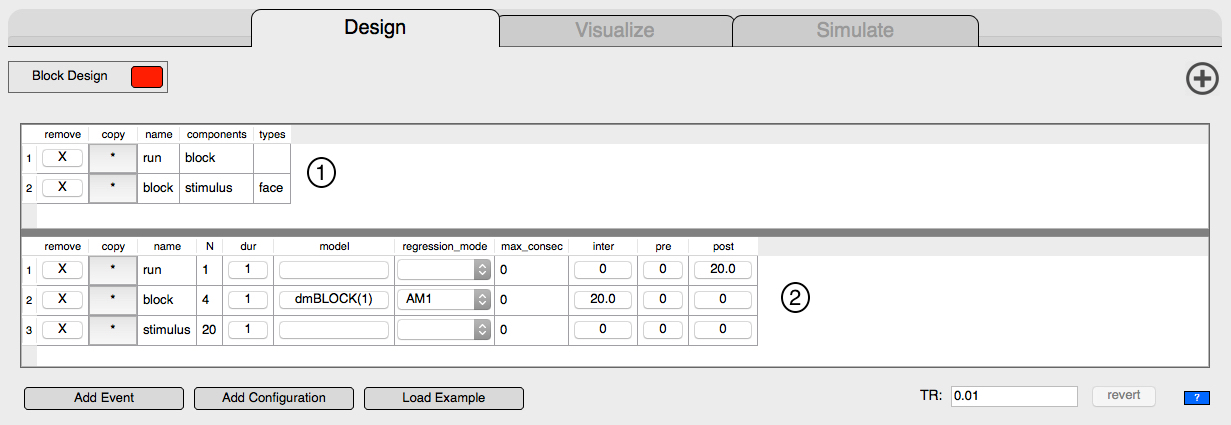
\includegraphics[width=0.95\textwidth,frame]{fig/12_block_config.jpg}
			\caption{Block design configuration}
			\label{fig:block_config}
		\end{figure}
		\begin{enumerate}
			\item Click the \textbf{New Design} button \nbut{}
			\item Enter ``Block Design'' as the name of the design, click \textbf{ok}
			\item Add two rows into the Event Definition table, Figure \hyperref[fig:block_config]{Figure \ref{fig:block_config}}, \circled{1}, using the \textbf{Add Event} button.
			\item \textbf{Name} the first row ``run'', and add a \textbf{component} called ``block''.
			\item \textbf{Name} the second row ``block'', add a \textbf{component} called ``stimulus'', with one \textbf{type} called ``face''.
			Thus, our event ``run'' will consist of ``block'' events which, in turn, will consist of ``stimulus'' events that have one type: ``face''.
			\item Now, configure the events in the Event Configuration table, \hyperref[fig:block_config]{Figure \ref{fig:block_config}}, \circled{2}: Add three rows using the \textbf{Add Configuration} button.
			\item \textbf{Name} the first row ``run''.
			You can keep the defaults except for the \textbf{post} column where you will enter a 20 second post-run fixation period.
			\item \textbf{Name} the second row ``block'' and set the number of blocks (\textbf{N}) to 4.
			This is the event with which we will want to model the hemodynamic response.
			In the \textbf{model} column, select ``dmBLOCK'' with an amplitude of 1.
			In the \textbf{regression\_mode} column, select ``AM1''.
			Finally, we want to make sure that there is a consistent rest period in between blocks.
			Set the \textbf{inter} column to equal 20 seconds.
			\item \textbf{Name} the third row ``stimulus''.
			Set the number of stimuli (\textbf{N}) to 20.
			We can keep the duration equal to 1 second, this makes our block duration equal to 20 seconds.
		\end{enumerate}
		\begin{figure}[ht]
			\centering
			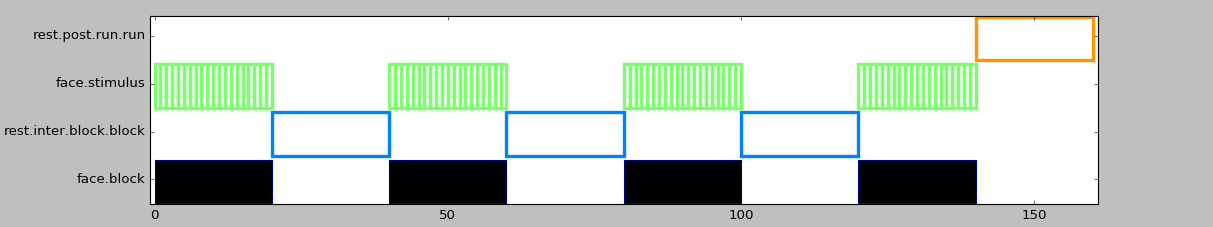
\includegraphics[width=0.70\textwidth,frame]{fig/13_block_event.jpg}
			\caption{Block design event plot}
			\label{fig:block_event_plot}
		\end{figure}
		After defining and configuring your events, your event plot should look like \hyperref[fig:block_event_plot]{Figure \ref{fig:block_event_plot}}.
		The \textcolor{green}{\textbf{green}} boxes show an individual presentation of a face (twenty per block).
		Compare this to the \textbf{black} box that corresponds to the block as a whole.
		This block is solid colored because this is the event we will use to model the hemodynamic response.
		Instead of estimating a response for each stimulus, we are estimating a response for each block.
		The \textcolor{blue}{\textbf{blue}} boxes are the 20 second inter-block fixation period and the \textcolor{orange}{\textbf{orange}} box corresponds to the 20 second post-run fixation block.
		While there are a few different events in this design, essentially we are telling the program that we want to alternate 20 seconds of stimulus with 20 seconds of rest.

	\subsection{Visualize Event Signal}
	\label{subsec:u3viz}
		Now that the experiment is constructed, we can see what the hemodynamic response would look like under ideal conditions.
		Change to the \textbf{Visualize} tab and click the \textbf{signal} button to see this response.
		Your response should look like \hyperref[fig:block_response_plot]{Figure \ref{fig:block_response_plot}}.
		\begin{figure}[ht]
			\centering
			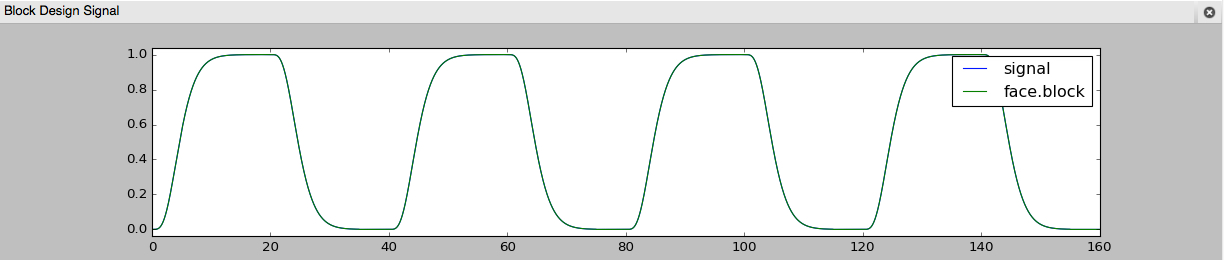
\includegraphics[width=0.70\textwidth,frame]{fig/14_block_viz_plot.jpg}
			\caption{Block design response plot}
			\label{fig:block_response_plot}
		\end{figure}
	\newpage

	\subsection{Unit Exercises}
	\label{subsec:u3exercises}
		\begin{enumerate}
			\item Change the TR to a more realistic 2 seconds, then an unrealistic 5, 10, and 20 seconds.
			How does the response change?
			\item Change the TR back to 2 seconds.
			Now lets make the rest blocks shorter: change the \textbf{inter} column of the block row from 20 to 10, 5, 1, and 0 seconds.
			How does the response change?
			\item Change the \textbf{inter}-block interval back to 20 seconds.
			Now return to the \hyperref[subsubsec:design]{design} tab and enter our control condition, scrambled, as another \textbf{type} of stimulus in the Event Definition table.
			How does the event plot change?
			Is this an ideal event ordering, why or why not?
			\item In the \textbf{Design} tab, change the \textbf{max\_consec} column to 1.
			This means that we want a maximum of one consecutive block per trial.
			Now, the experiment should alternate blocks by condition.
			Return to the \textbf{Visualize} tab, and view the \textbf{signal}.
			As in question 2, change the \textbf{inter}-block interval from 20 to 10, 5, 1, and 0.
			What happens as the inter-block interval gets smaller and why might this spell trouble for our statistical analyses? 
			\item Now, create an all new design (\nbut{}).
			Call this experiment whatever you want.
			In this experiment you will show your participants threatening pictures (i.e. someone pointing a gun at the camera) and a control condition.
			Your experiment should have the following hierarchy:
		\begin{figure}[ht]
			\centering
			\begin{scaletikzpicturetowidth}{\textwidth}
			\begin{tikzpicture}[scale=\tikzscale]
				\Tree 
	 			[ .{experiment}
	 				[ .{run}
	   					[ .{block} 
	     						[ .{threat} ]
	     						[ .{threat} ]
	     						[ .{threat} ]
	     						[ .{threat} ] ]
						[ .{rest} 
							[ .{rest} ]
	     						[ .{rest} ]
	     						[ .{rest} ]
	     						[ .{rest} ] ]
						[ .{block} 
	     						[ .{control} ]
	     						[ .{control} ]
	     						[ .{control} ]
	     						[ .{control} ] ] 
						[ .{post} ] ]
					[ .{run}
	   					[ .{block} 
	     						[ .{threat} ]
	     						[ .{threat} ]
	     						[ .{threat} ]
	     						[ .{threat} ] ]
						[ .{rest} 
							[ .{rest} ]
	     						[ .{rest} ]
	     						[ .{rest} ]
	     						[ .{rest} ] ]
						[ .{block} 
	     						[ .{control} ]
	     						[ .{control} ]
	     						[ .{control} ]
	     						[ .{control} ] ] 
						[ .{post} ] ] ]
			\end{tikzpicture}
			\end{scaletikzpicturetowidth}
			\label{fig:block_heirarchy_exerecise}
		\end{figure} \\
		With respect to event timing, each task and rest block should be 15 seconds long.
		Each run should consist of 10 task blocks and there should be no more than 1 consecutive block per trial.
		In addition, add a post-run fixation period of 15 seconds.
		Tell the program to model the hemodynamic response of the entire block length same as in \hyperref[subsec:u3define]{section \ref{subsec:u3define}}.
		\end{enumerate}
\newpage

%%%%%%%%%%%%%%%%%%%%%%%%%%%%
%%%%%%%%%% Unit 4 %%%%%%%%%%
%%%%%%%%%%%%%%%%%%%%%%%%%%%%

\section{Unit 4: Slow Event Related Designs}
\label{sec:unit4}
	\subsection{Overview}
	\label{subsec:u4overview}
		The previous unit explored the powerful fMRI design known as block designs. 
		In this type of design, you take advantage of the fact that the BOLD signal scales linearly with the amount of stimuli, that is, more stimuli in a quick period of time will give stronger BOLD response (if the brain region in question is actually responsive to the stimulus) compared to baseline.
		While this design is effective at generating large differences in the amplitude of the BOLD response, there are some drawbacks.
		As we saw, for a block design to elicit the strongest difference in response, there needs to be adequate time for the response to return to baseline.
		Block designs are less about the response to an individual stimulus and more in line with the summation of many stimuli.
		Another type of design, event related, allows for multiple stimulus presentations while estimating the hemodynamic response of individual stimuli.
		This unit will focus on slow event related designs, which allows the hemodynamic response to return to baseline.

	\subsection{The Design}
	\label{subsec:u4design}
		Initially, we will construct a flexible, but simple, slow event-related design to which we will later add complexity.
		We will continue to address our research question: where in the brain are responses stronger to faces compared to other stimuli?
		The event hierarchy of the experiment will look like \hyperref[fig:slow_event_heirarchy]{Figure \ref{fig:slow_event_heirarchy}}.
		Once difference between this design and the previous unit will be that the duration of the stimulus presentation (face events) and the duration of the ITI (rest) will not be equal.
		The stimulus presentation (i.e. face events) will consist of transient, 1 second, presentations whereas the ITI events will allow the hemodynamic response to return to baseline after estimating the response to a single stimulus event.
		\begin{figure}[ht]
			\centering
			\begin{scaletikzpicturetowidth}{0.5\textwidth}
			\begin{tikzpicture}[scale=\tikzscale]
				\Tree 
	 			[ .{experiment}
	 				[ .{run}
						[ .{trial}
							[ .{face} ]
							[ .{iti} ] ]
						[ .{trial}
							[ .{face} ]
							[ .{iti} ] ]
						[ .{trial}
							[ .{face} ]
							[ .{iti} ] ]
	     					[ .{trial}
							[ .{face} ]
							[ .{iti} ] ]
	     					[ .{trial}
							[ .{face} ]
							[ .{iti} ] ]
	     					[ .{trial}
							[ .{face} ]
							[ .{iti} ] ] ] 
						[ {post} ] ]
			\end{tikzpicture}
			\end{scaletikzpicturetowidth}
			\caption{Slow event hierarchy}
			\label{fig:slow_event_heirarchy}
		\end{figure}

	\subsection{Define and Configure Events}
	\label{subsec:u4define}
		We will define our events similar to the previous unit, with some important differences:
		\begin{figure}[ht]
			\centering
			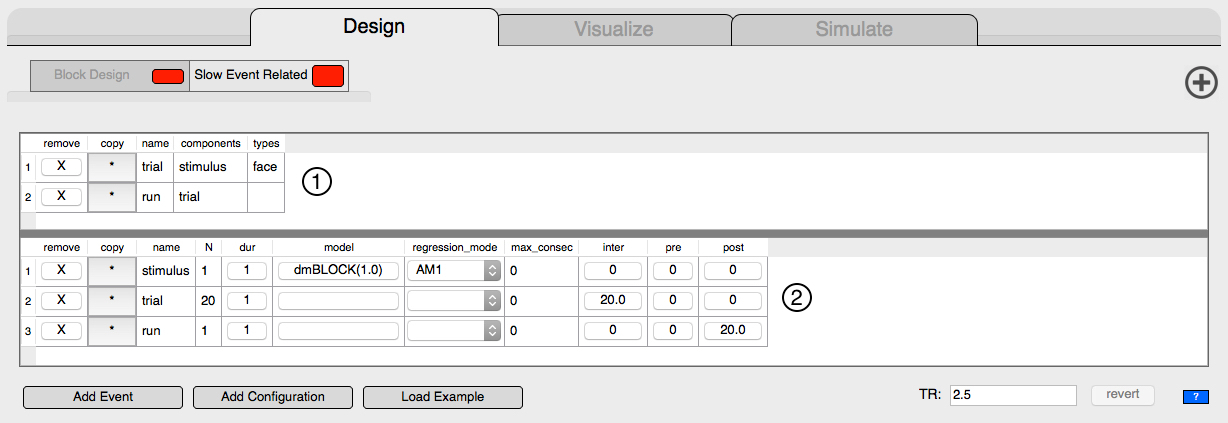
\includegraphics[width=0.95\textwidth,frame]{fig/15_slow_event_config.jpg}
			\caption{Initial Slow event related configuration}
			\label{fig:slow_event_config}
		\end{figure}
		\begin{enumerate}
			\item Using the \textbf{Add Event} button, add a row into the Event Definition table (\hyperref[fig:slow_event_config]{Figure \ref{fig:slow_event_config}}, \circled{1}). Add an event called ``run'' with a \textbf{component} called ``trial''.
			\item Add another row called trial with a \textbf{component} called ``stimulus'' with only one \textbf{type} called ``face''.
			\item Using the \textbf{Add Configuration} button, add an event into the Event Configuration table (\hyperref[fig:slow_event_config]{Figure \ref{fig:slow_event_config}}, \circled{2}) called ``run''.
			We can use all of the defaults but, as before, we will enter a post run fixation of 20 seconds.
			\item Add a row called ``trial'', keep the defaults except for the number of events (\textbf{N}) in which we will add 20 events and change the inter-trial interval (ITI) to a constant 20 seconds.
			\item Add another row called ``stimulus'', keep the defaults except that this is the event where we will want to estimate a hemodynamic response.
			Under the \textbf{model} column select the \textbf{dmBLOCK} model with an amplitude of 1.
			Also, in the \textbf{regression\textunderscore mode} column, select \textbf{AM1}.
			\item We can keep the TR at 2.5 seconds.
		\end{enumerate}
			Once all events are defined and configured your event plot should look like \hyperref[fig:slow_event_plot]{Figure \ref{fig:slow_event_plot}}.
			Each run (we have only prescribed one, for now) will consist of smaller events called trials.
			Within each trial there will always be two smaller events: a stimulus and an associated ITI.
			The stimulus event will be the presentation of the stimulus (e.g. a face) and the ITI event is an accompanying period of rest that allows the hemodynamic response to return to baseline.
			Of note in \hyperref[fig:slow_event_plot]{Figure \ref{fig:slow_event_plot}} is the solid event denoted \textbf{face.stimulus}.
			These are the events that will serve as the basis for the estimation of the hemodynamic response.
			The \textcolor{green}{\textbf{green}} box denotes the ITI, whereas the \textcolor{blue}{\textbf{blue}} box denotes the face trial.
			This block box is colored as an empty box, however, the event is so short that the box does not look empty.
			\begin{figure}[ht]
				\centering
				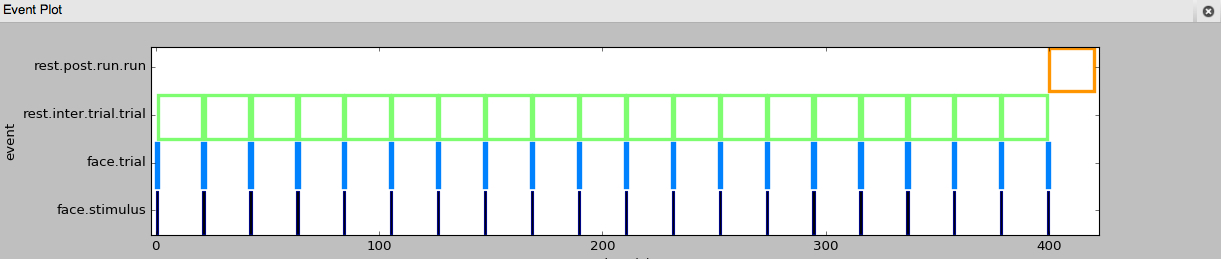
\includegraphics[width=0.70\textwidth,frame]{fig/16_slow_event_event.jpg}
				\caption{Initial slow event related event plot}
				\label{fig:slow_event_plot}
			\end{figure}

		\subsection{Visualize Event Signal}
		\label{subsec:u4viz}
			To view the response plots, click the \hyperref[subsubsec:visualize]{Visualize} tab.
			You will see the \hyperref[subsubsec:visualize]{Visualize} tab's Event Configuration table which corresponds to table you configured in the previous step.
			As in the previous unit, you will edit the event parameters and explore the changes in the hemodynamic response plots.
			Click the \textbf{signal} button to see the response plot.
			You initial response plot should look like \hyperref[fig:slow_event_response]{Figure \ref{fig:slow_event_response}}.
			\begin{figure}[ht]
				\centering
				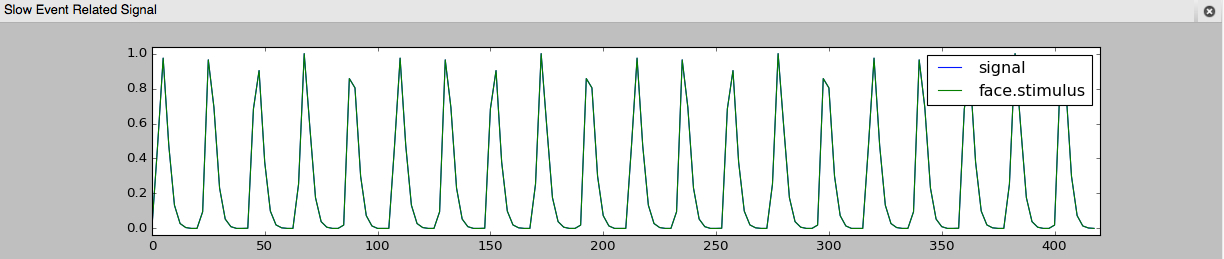
\includegraphics[width=0.70\textwidth,frame]{fig/17_slow_event_viz_plot.jpg}
				\caption{Initial slow event related response plot}
				\label{fig:slow_event_response}
			\end{figure}
	\newpage

	\subsection{Unit Exercises}
	\label{subsec:u4exercises}
		\begin{enumerate}
			\item Change the duration of the \textbf{ITI} from 20 to 15, 10, 5, 3, 2, 1, and 0. How does the signal change in amplitude and shape? Why?
			\item Set the duration of the \textbf{ITI} back to 20 seconds.
			Now lets add our control condition from the previous unit: scrambled.
			Return to the \textbf{Design} tab and enter another \textbf{type} of trial called scrambled into the Event Definition table (\textbf{Figure 6}, \circled{1}).
			How did the event plot at the bottom of the \textbf{Design} tab change from \hyperref[fig:slow_event_plot]{Figure \ref{fig:slow_event_plot}} ?
			\item How did the response plot in the \textbf{Visualize} tab change with the addition of the second condition? 
			Change the duration of the \textbf{ITI} from 20 to 15, 10, 5, 3, 2, 1, and 0. 
			When do the event-specific peaks in the response begin to disappear?
			\item What is one reason that a long ITI of 20 seconds would be good to disentangle the relative contribution of each condition to the overall signal? \textbf{HINT:} think about the time course of the hemodynamic response
		\end{enumerate}
\newpage

%%%%%%%%%%%%%%%%%%%%%%%%%%%%
%%%%%%%%%% Unit 5 %%%%%%%%%%
%%%%%%%%%%%%%%%%%%%%%%%%%%%%

\section{Unit 5: Assessing Design Quality}
\label{sec:unit5}
	\subsection{Overview}
	\label{subsec:u5overview}
		In addition to visualizing the event and signal structure of your design, the Design Explorer also gives you the ability to quantify design quality and compare to this quality to other designs.
		It is essential to quantitatively evaluate your design because you will not be able to choose an ideal timing based on visual inspection alone.
		This unit will focus on how to define and assess design quality.

	\subsection{Optimization}
	\label{subsec:u5optimization}
		One feature of the Design Explorer is that it gives you the ability to optimize your experimental design based on design quality.
		This feature allows the computer to generate a random stimulus order and timing (with the constraints specified by the user) and compare quality metrics to choose the best timing.
		In order to compare the quality of multiple designs, each design should be optimized before examining the quality metrics.
		The program uses a \textcolor{red}{\textbf{red}} box to denote designs that need to be optimized and a \textcolor{green}{\textbf{green}} box to denote designs that have been optimized. \\
		\begin{figure}[ht]
			\centering
			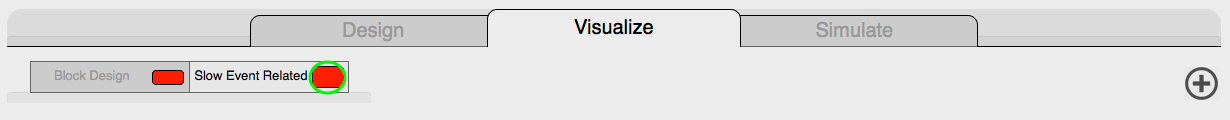
\includegraphics[width=0.95\textwidth,frame]{fig/18_design_optimize_button.jpg}
			\caption{How to optimize}
			\label{fig:select_optimize}
		\end{figure}
		\begin{wrapfigure}{r}{0.45\textwidth}
			\centering
			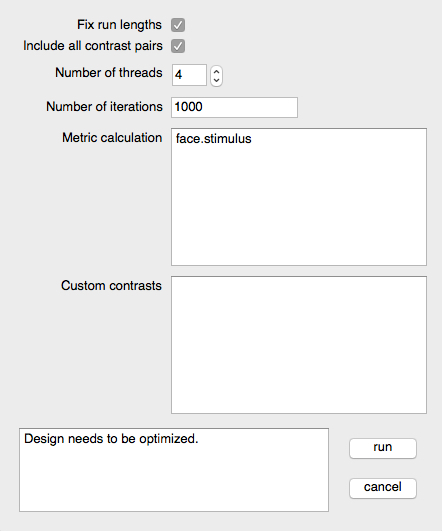
\includegraphics[width=.4\textwidth,frame]{fig/19_optimize_menu.jpg}
			\caption{Optimization window}
			\label{fig:optimize}
		\end{wrapfigure} \\
		To optimize:
		\begin{enumerate}
			\item Click on the \textcolor{red}{\textbf{red}} box of the design you wish to optimize (\hyperref[fig:select_optimize]{Figure \ref{fig:select_optimize}}, \textcolor{green}{\textbf{green}} circle) - this will open the optimize window (\hyperref[fig:optimize]{Figure \ref{fig:optimize}}).
			\item You can keep the defaults for now, but this window gives you the ability to customize your optimization.
			However, make sure you set the number if \textbf{iterations} to a sufficiently high number.
			For the purposes of this workbook, 1000 is good, but if you are fully optimizing a real study, you should choose a very large number like 10,000 or 100,000.
			1000 iterations on a 2-core machine Macbook Pro takes about 40 seconds.
			\item Click \textbf{run} to run the optimization.
			In the terminal window, you should see the iteration number.
			Once the optimization is finished, the optimization window will disappear and the optimization box will change to \textcolor{green}{\textbf{green}}.
		\end{enumerate}

	\subsection{Quality Metrics}
	\label{subsec:u5qualmet}
		The following are quantitative measures that can tell you different things about the quality of your design, remember that do accurately compare designs, you must optimize the timing first.
		\begin{description}
			\item{\textbf{Normalized Standard Deviation}}:
				Normalized standard deviation refers to the standard deviation in your beta estimates from the linear regression. You want the normalized standard deviation to be as small as possible, the smaller the uncertainty in your beta estimates, the better.
				This metric gives you a normalized standard deviation for each modeled event.
			\item{\textbf{Metric Quality}}: This quantitative measure of design quality summarizes the normalized standard deviation for all events provided in the \textbf{metric} list during optimization.
				Thus, there is only one value per design.
				Optimization is required to examine this measure.
				Because this number summarizes the normalized standard deviation of the beta estimates, the lower this is the better.
			\item{\textbf{Collinearity}}: This is the correlation between the time series of different events.
				For all events, you want the collinearity to be as small as possible.
			\item{\textbf{Variance Inflation Factor (VIF)}}: When there is a strong correlation between two events (i.e. say one event always follows another), also called collinearity, it becomes difficult to disentangle the relative influence of each individual event. 
				The VIF is a measure of how much the variance of an estimated beta coefficient increases because of collinearity. You want the VIF to be as small as possible, as well.
		\end{description}
		\begin{figure}[ht]
			\centering
			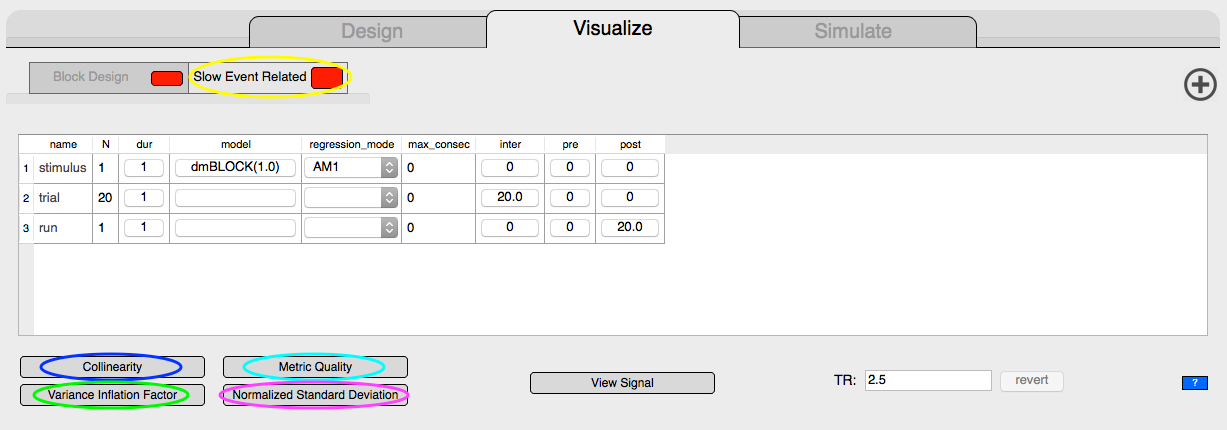
\includegraphics[width=0.95\textwidth,frame]{fig/20_viz_quality_metrics.jpg}
			\caption{Visualize Quality Measures}
			\label{fig:slow_quality}
		\end{figure}
		To visualize the metric quality, click on the \textbf{metric quality} button (\textcolor{Cyan}{\textbf{cyan}} circle).
		To visualize the collinearity metric, click on the \textbf{collinearity} button (\textcolor{blue}{\textbf{blue}} circle).
		To visualize a histogram of the VIF, click on the \textbf{variance inflation factor} button (\textcolor{green}{\textbf{green}} circle).
		To visualize the normalized standard deviation metric, click on the \textbf{normalized standard deviation} button (\textcolor{Magenta}{\textbf{magenta}} circle).
		In the next section we will create two different designs and compare the quality measures.

	\subsection{Compare Designs}
	\label{subsec:u5compare}
		Now we are in position to examine how small changes can quantitatively affect the quality of an experimental design.
		To do this, we first need to have 2 similar variants to which we can compare:
		\begin{enumerate}
			\item Right click on your Slow Event Related design tab, \hyperref[fig:slow_quality]{Figure \ref{fig:slow_quality}}, \textcolor{Goldenrod}{\textbf{yellow}} circle.
			\item Select \textbf{copy}
			\item You can keep the default design name (Slow Event Related (2)).
			This will duplicate this variant so that you can change one parameter and compare.
			\item We no longer need the Single Event design, so you can delete it:
			\begin{enumerate}
				\item Right click on the Single Event tab
				\item Select \textbf{delete}
			\end{enumerate}
			\item Make sure you optimize each of these designs using 1000 iterations.
		\end{enumerate}
		Your \textbf{Design toolbar} should now look like \hyperref[fig:two_designs]{Figure \ref{fig:two_designs}}: \\
		\begin{figure}[ht]
			\centering
			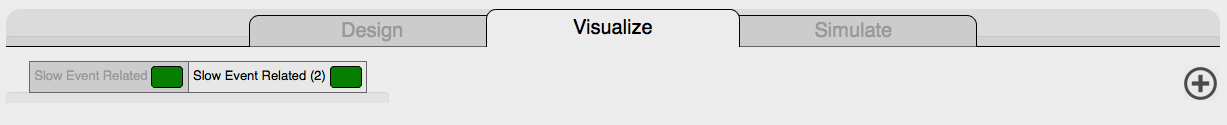
\includegraphics[width=0.95\textwidth,frame]{fig/21_optimized_designs.jpg}
			\caption{Design toolbar with copied designs}
			\label{fig:two_designs}
		\end{figure} \\
		Now, in the \textbf{Visualize} tab, lets compare the VIF of both designs (Figure~\ref{fig:VIF} \textcolor{green}{green} circle):
		\begin{figure}[ht]
			\centering
			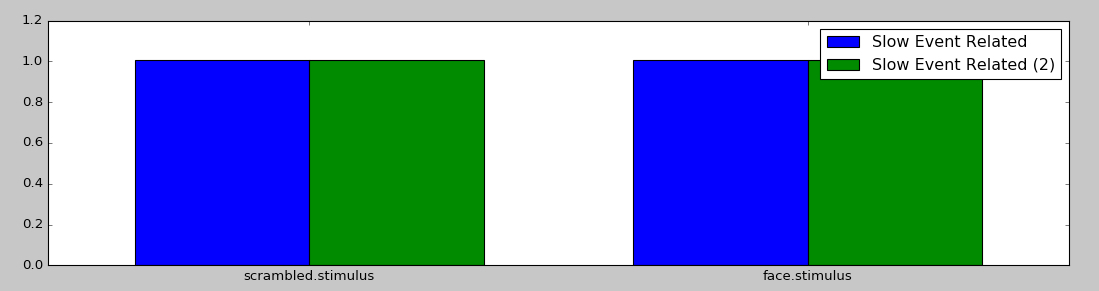
\includegraphics[width=\textwidth,frame]{fig/22_VIF.jpg}
			\caption{Variance inflation factor}
			\label{fig:VIF}
		\end{figure} \\
		It appears as though the VIF is the same for both designs.
		This makes sense because they are exactly the same, we haven't changed anything yet.
		\newpage

	\subsection{Unit Exercises}
	\label{subsec:u5exercises}
		\begin{figure}[ht]
			\centering
			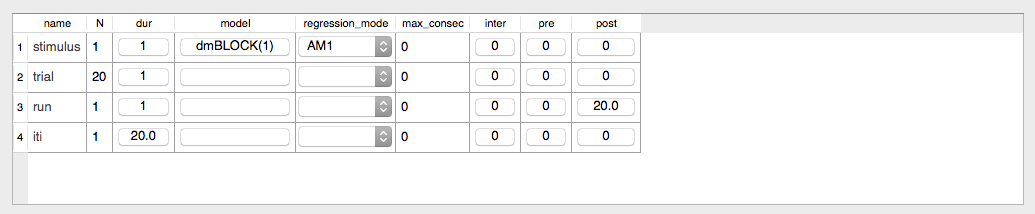
\includegraphics[width=0.95\textwidth,frame]{fig/23_VIF_ex.jpg}
			\caption{VIF exercises event configuration}
			\label{fig:VIF_ex}
		\end{figure}
		For the following exercises, ensure that both of your Slow Event Related variants look like \hyperref[fig:VIF_ex]{Figure \ref{fig:VIF_ex}}.
		We will keep the original variant the same (Slow Event Related) and alter the copy (Slow Event Related (2)).
		Make sure that after every alteration in parameters that you re-optimize the design for a proper comparison. \\
		Also, make sure your TR is set to 2.5 seconds and then proceed to the following exercises:
		\begin{enumerate}
			\item Change the \textbf{ITI} on Slow Event Related (2) to 15, 10, 5, and 1 second. How does making the ITI shorter affect the VIF and the metric quality?
			\item How does the response plot change with the shorter ITI and what does this mean in the context of how the VIF changes?
			\item Chane the \textbf{ITI} back to 20 seconds. How does making the \textbf{stimulus} duration longer affect the VIF and metric quality? Why? Test with a stimulus duration of 5, 10, 20, and 30 seconds.
		\end{enumerate}
\newpage

%%%%%%%%%%%%%%%%%%%%%%%%%%%%
%%%%%%%%%% Unit 5 %%%%%%%%%%
%%%%%%%%%%%%%%%%%%%%%%%%%%%%

\section{Unit 6: Fast Event-Related}
\label{sec:unit6}
	\subsection{Overview}
	\label{subsec:u6overview}
		In the previous section, we learned how to construct and test the quality of a slow event related design.
		Slow event related designs are nice because they give the hemodynamic response a chance to return to baseline (or almost, depending on the duration of the ITI, as you saw).
		However, an MRI scan is very expensive and we want to make sure that we are efficient with the time.
		In addition, we want to make sure that we have enough stimulus presentations per condition to have enough power for statistical analysis.
		This section will explore how we can speed up stimulus timing while still trying to maximize experimental quality.
		To begin, we will construct an experiment with similar hierarchy as in Unit 4 (Slow Event Designs), see \hyperref[fig:fast_hierarchy]{Figure \ref{fig:fast_hierarchy}}.
		In this hierarchy, ``scram'' is short for scrambled.
		The major difference between this design and the design in Unit 4 is that the timing between events will be much faster (which is not apparent in the \hyperref[fig:fast_hierarchy]{Figure \ref{fig:fast_hierarchy}}, but will be more clear as we configure our events).
		\begin{figure}[ht]
			\centering
			\begin{scaletikzpicturetowidth}{0.6\textwidth}
			\begin{tikzpicture}[scale=\tikzscale]
				\Tree 
	 			[ .{experiment}
	 				[ .{run}
						[ .{trial}
							[ .{face} ]
							[ .{rest} ] ]
						[ .{trial}
							[ .{scram} ]
							[ .{rest} ] ]
						[ .{trial}
							[ .{face} ]
							[ .{rest} ] ]
	     					[ .{trial}
							[ .{scram} ]
							[ .{rest} ] ]
	     					[ .{trial}
							[ .{face} ]
							[ .{rest} ] ]
	     					[ .{trial}
							[ .{scram} ]
							[ .{rest} ] ] ] 
						[ {post} ] ]
			\end{tikzpicture}
			\end{scaletikzpicturetowidth}
			\caption{Fast event hierarchy}
			\label{fig:fast_hierarchy}
		\end{figure}

	\subsection{Define and Configure Events}
	\label{subsec:u6define}
		Now lets define this in the Design Explorer.
		Your Event Definition and Event Configuration tables should look like the tables in \hyperref[fig:fast_event_config]{Figure \ref{fig:fast_event_config}}.
		\begin{figure}[ht]
			\centering
			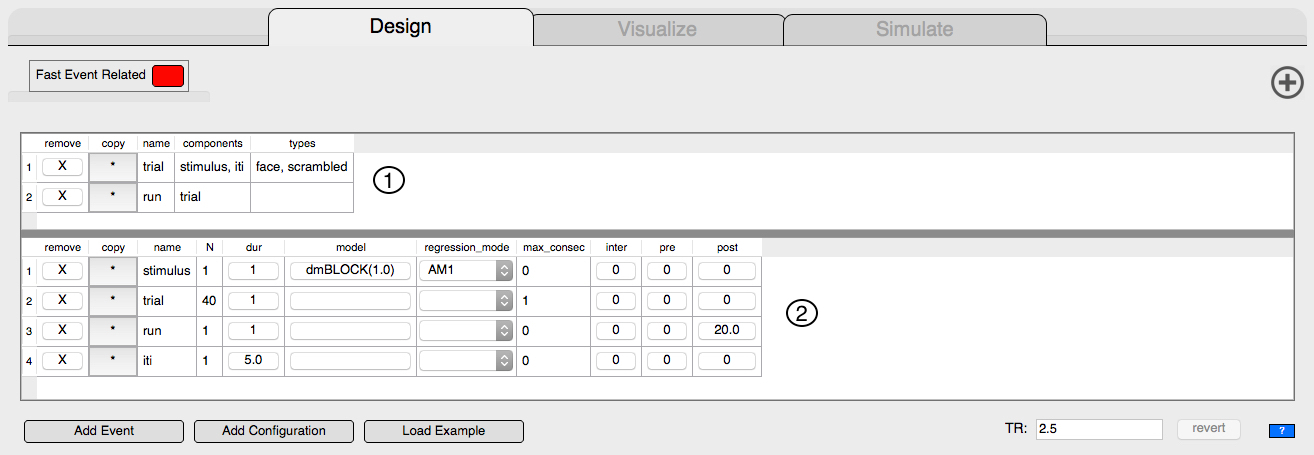
\includegraphics[width=.95\textwidth,frame]{fig/24_fast_event_config.jpg}
			\caption{Initial Fast event related configuration}
			\label{fig:fast_event_config}
		\end{figure}
		\begin{enumerate}
			\item Create a new design, call this ``Fast Event Related''
			\item Using the \textbf{Add Event} button, add a row into the Event Definition table.
			The \textbf{name} of this event will be ``run'' with a component called ``trial''.
			\item Add another row into the Event Definition table called ``trial'' with components called ``stimulus,iti'' and two \textbf{type}s called ``face,scrambled''.
			\item Now we'll configure the events. Use the \textbf{Add Configuration} button to add a row into the Events Configuration table.
			\item \textbf{Name} this event ``run'' and keep the default parameters.
			\item Add another row and \textbf{name} it ``trial''.
			Set the number of trials (\textbf{N}) to ``40''.
			Also, for the beginning of this example, lets set the \textbf{max\_consec} column to ``1'' - this means that there will be no more than 1 consecutive trial type (face and scrambled will always alternate).
			\item Add another row and \textbf{name} it ``stimulus''.
			Set the \textbf{model} to ``dmBlock'' with an amplitude of 1.
			Set the \textbf{regression\_mode} to ``AM1''.
			\item Finally, add a row \textbf{named} ``iti'' and change the duration (\textbf{dur}) to 10 seconds.
		\end{enumerate}
		When you are finished, your event plot should look like \hyperref[fig:fast_event_plot]{Figure \ref{fig:fast_event_plot}}.
		\begin{figure}[ht]
			\centering
			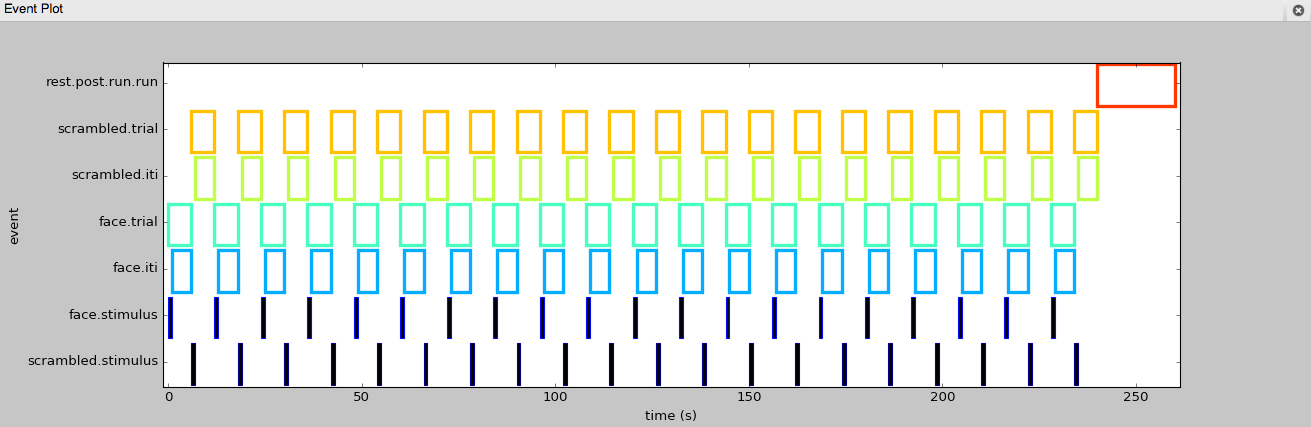
\includegraphics[width=0.70\textwidth,frame]{fig/25_fast_event_event.jpg}
			\caption{Initial fast event related event plot}
			\label{fig:fast_event_plot}
		\end{figure}

	\subsection{Visualize Events}
	\label{subsec:u6viz}
		\begin{figure}[ht]
			\centering
			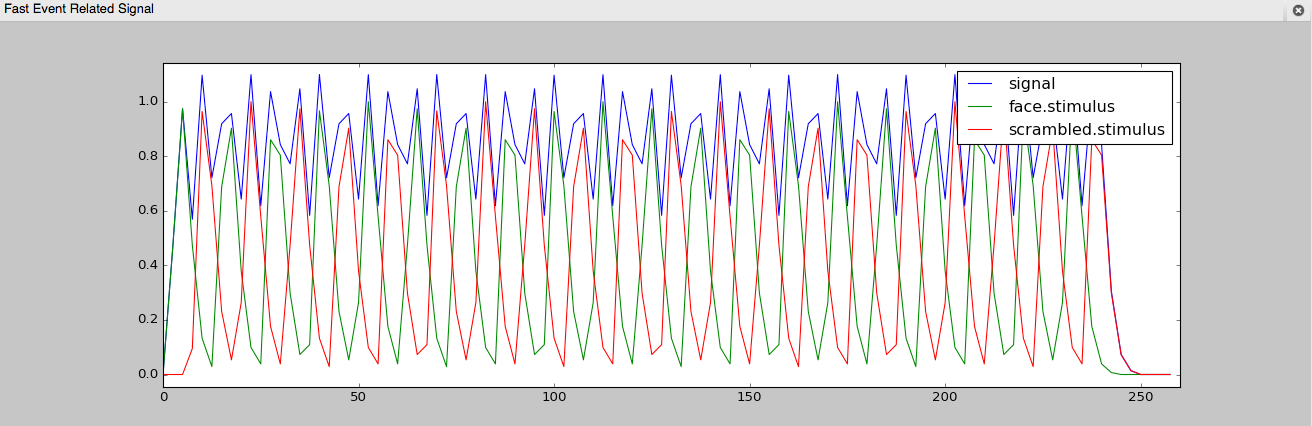
\includegraphics[width=0.70\textwidth,frame]{fig/26_fast_event_viz_plot.jpg}
			\caption{Fast event related signal}
			\label{fig:fast_event_signal}
		\end{figure}
		Once your experiment is constructed, the \textbf{signal} in the \textbf{visualize} tab should look like \hyperref[fig:fast_event_signal]{Figure \ref{fig:fast_event_signal}}.
		The \textcolor{green}{\textbf{green}} line corresponds to the signal specific to the face condition whereas the \textcolor{red}{\textbf{red}} line corresponds to the signal specific to the scrambled condition.
		The \textcolor{blue}{\textbf{blue}} line corresponds to the sum of the two conditions, which would be the ideal hemodynamic response.
	\newpage

	\subsection{Unit Exercises}
	\label{subsec:u6exercises}
		Since we initially constrained the trials to alternated, there is no need to optimize the design because there are only two, equal, solutions (face,scrambled; scrambled,face).
		However, set \textbf{max\_consec} to 2 so that the trial order can vary.
		No you can properly optimize trial order based on the prescribed stimulus timing and do the following exercises.
		\begin{enumerate}
			\item Create a copy of the fast event design variant, and change the ITI duration (\textbf{dur}) to a jittered duration (\textbf{uni} option) with a lower bound of 3 seconds and an upper bound of 7 seconds.
			Make sure each design is optimized using 1000 iterations.
			How does the VIF and metric quality change between these two designs?
			\item Make the designs equal again by setting the jitter back to a constant 5 second ITI.
			How does changing the \textbf{max\_consec} option to 2 in one of the experiments change the metric quality and VIF?
		\end{enumerate}

% \newpage
% \section{Load Examples}
% 	To aid the exploration of how changes in experimental design can lead to quantitative differences in quality metrics, the Design Explorer has a number of example templates that can be quickly loaded.
% 	This way, you can quickly load a template and efficiently explore different types of designs.

% 	\vspace{3mm}
% 	% \begin{figure}[ht]
% 	% 	\centering
% 	% 	\includegraphics[width=.9\textwidth,frame]{blank_window_example.jpg}
% 	% 	\caption{Load example}
% 	% 	\label{fig:load_example}
% 	% \end{figure}

% 	To load an example: \\
% 	\begin{enumerate}
% 		\item Click on the \textbf{load example} button (Figure~\ref{fig:load_example}, \textcolor{blue}{\textbf{blue}} circle).
% 		\item In the \textbf{choose example} window, enter a number (1-4).
% 		See the table below for which design each number corresponds to.
% 		\item Click \textbf{ok}.
% 	\end{enumerate}

% 	\vspace{10mm}
% 	\begin{center}
% 	\begin{tabular}{ c c }
% 		Number 	& 	Design Type \\
% 		\hline
% 		1 	& 	Block \\
% 		2 	& 	Slow Event Related \\
% 		3 	& 	Fast Event Related \\
% 		4 	& 	Monetary Incentive Delay
% 	\end{tabular}
% 	\end{center}		

% \newpage
% \section{Unit 7: Signal and Noise}








\end{document}




